\section{Background Prediction and Validation}
\label{sec:BackgroundEstimation}

In this section the strategies for  the prediction of the background contributions and validation of these predictions are described.
Monte Carlo  simulation is extensively used to model the kinematical properties of the signal and background processes.
However, since the  simulation is prone to systematic
uncertainties due to a non-perfect description of pileup effects, the
underlying event and the detector performance, the  QCD multi-jet and $\Ztautau$ 
background contributions are estimated using dedicated signal-free control data samples 
as described  in sections~\ref{sec:qcd} and~\ref{sec:ztau}.
%estimate backgrounds from data. In particular for the following cases:
%\begin{itemize}
%  \item[$\bullet$] The $Z \rightarrow \tau\tau \rightarrow ll ~ + ~  4\nu$ is estimated from data using the embedding technique described in Section~\ref{sec:data_mc}.
%  \item[$\bullet$] The multi-jet background is estimated completely from data using the so-called ABCD method.   
%\end{itemize}
The contributions of the other background processes, such as \ttbar, single top quark, diboson, $Z
\rightarrow ll$ + jets (where $l = e,\mu$) and W + jets, are estimated
from simulation. Because of  the relatively large contribution of \ttbar background, a study to validate
this background prediction has been performed as described in section~\ref{sec:top_est}.

Good agreement between data and background prediction is found after the common selection as can be seen in 
Figures~\ref{fig:selections} and~\ref{fig:validation}.


\begin{figure}[p]
     \begin{center}
            %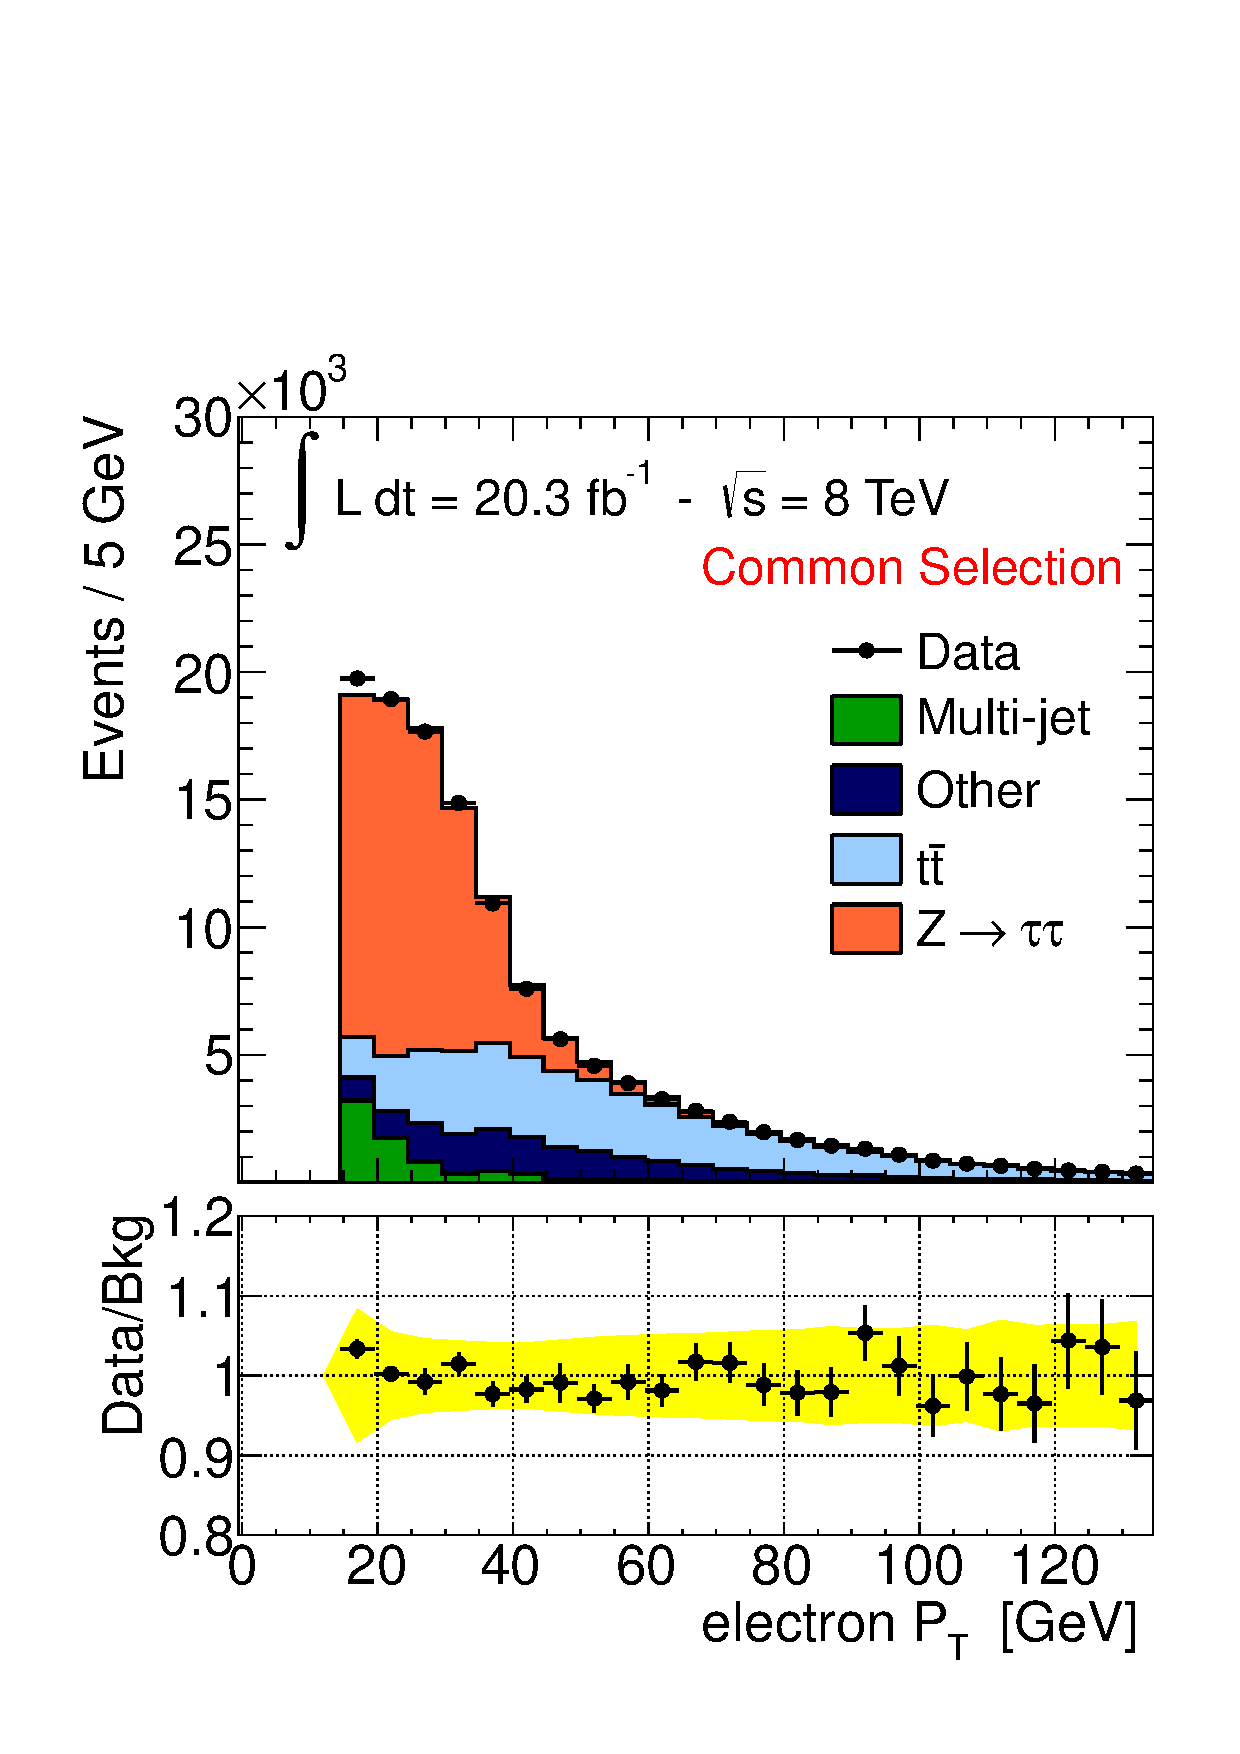
\includegraphics[width=0.47\textwidth]{figure/final_plots/std_presel_ele_pt.pdf}
            %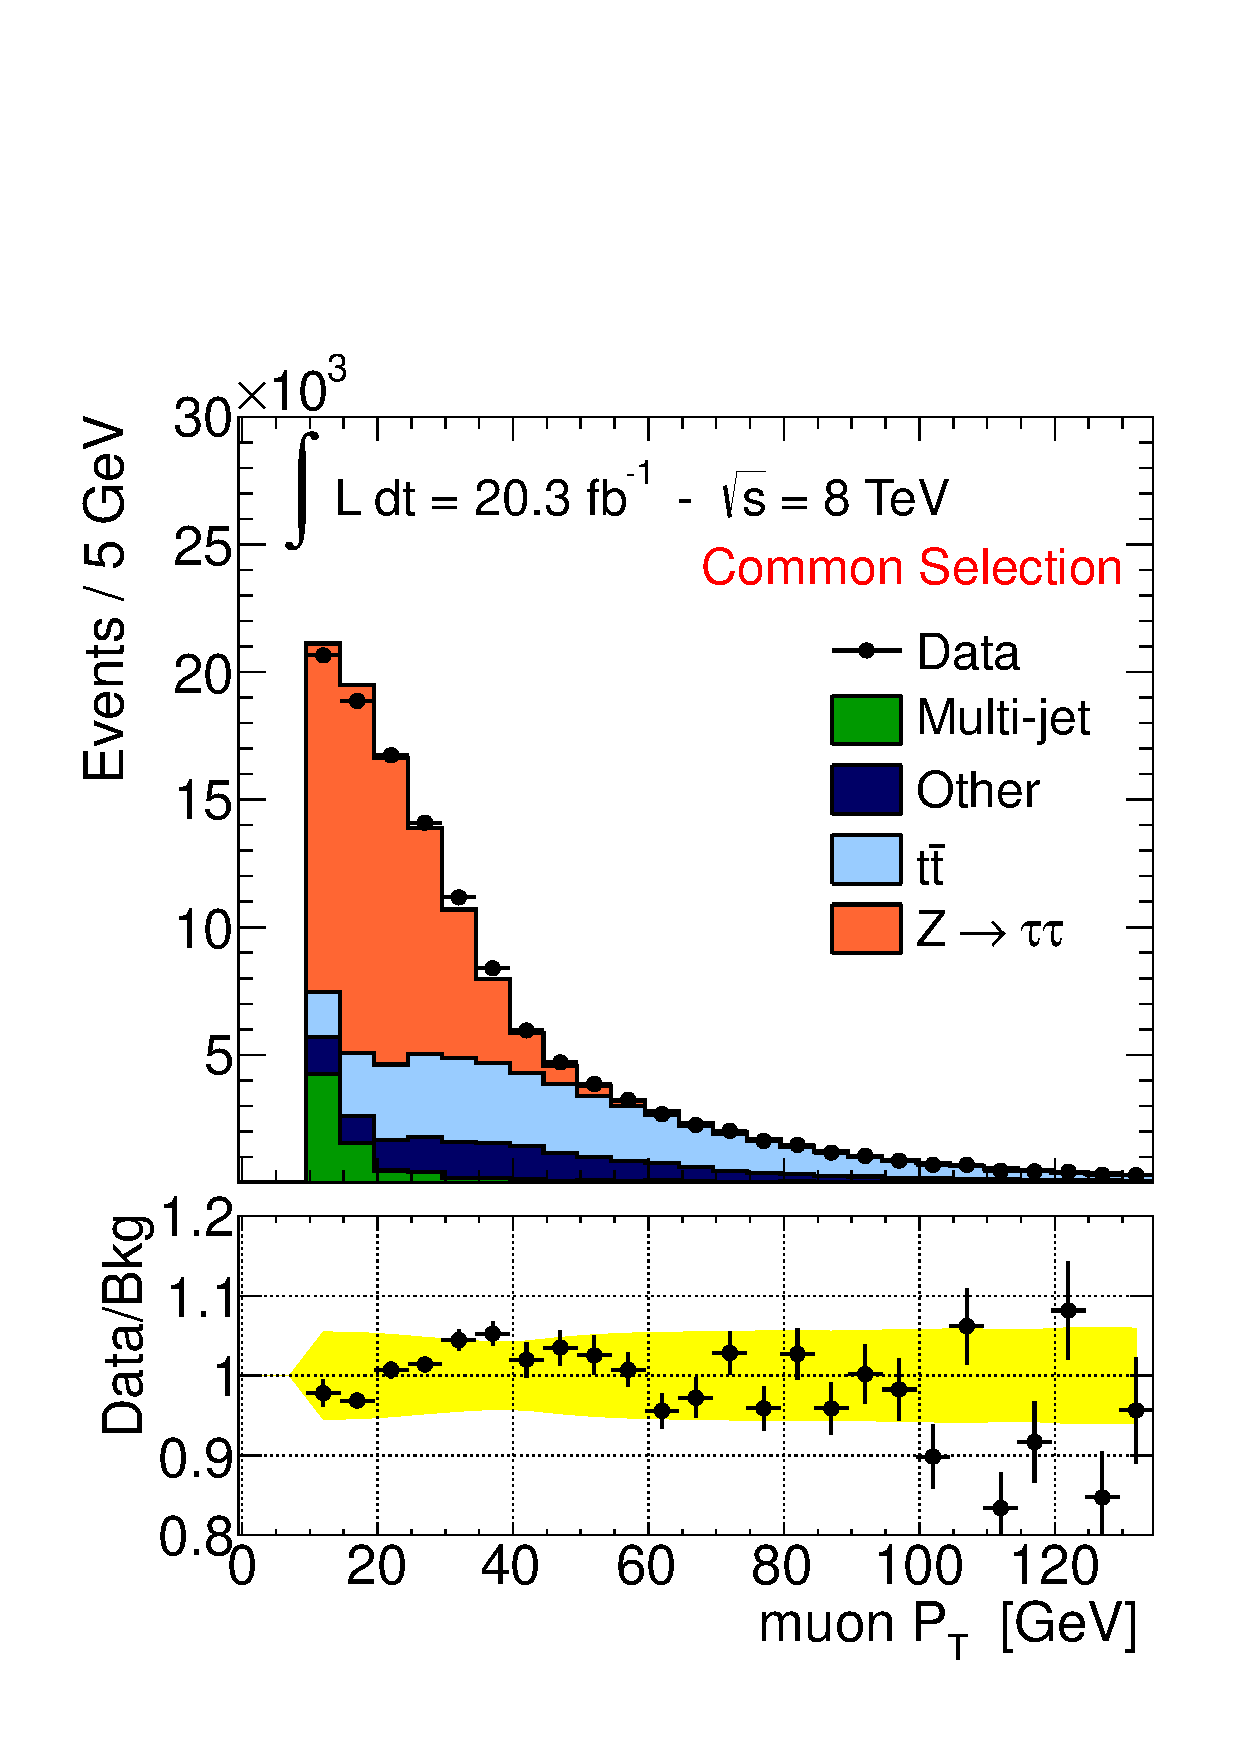
\includegraphics[width=0.47\textwidth]{figure/final_plots/std_presel_muon_pt.pdf}
            %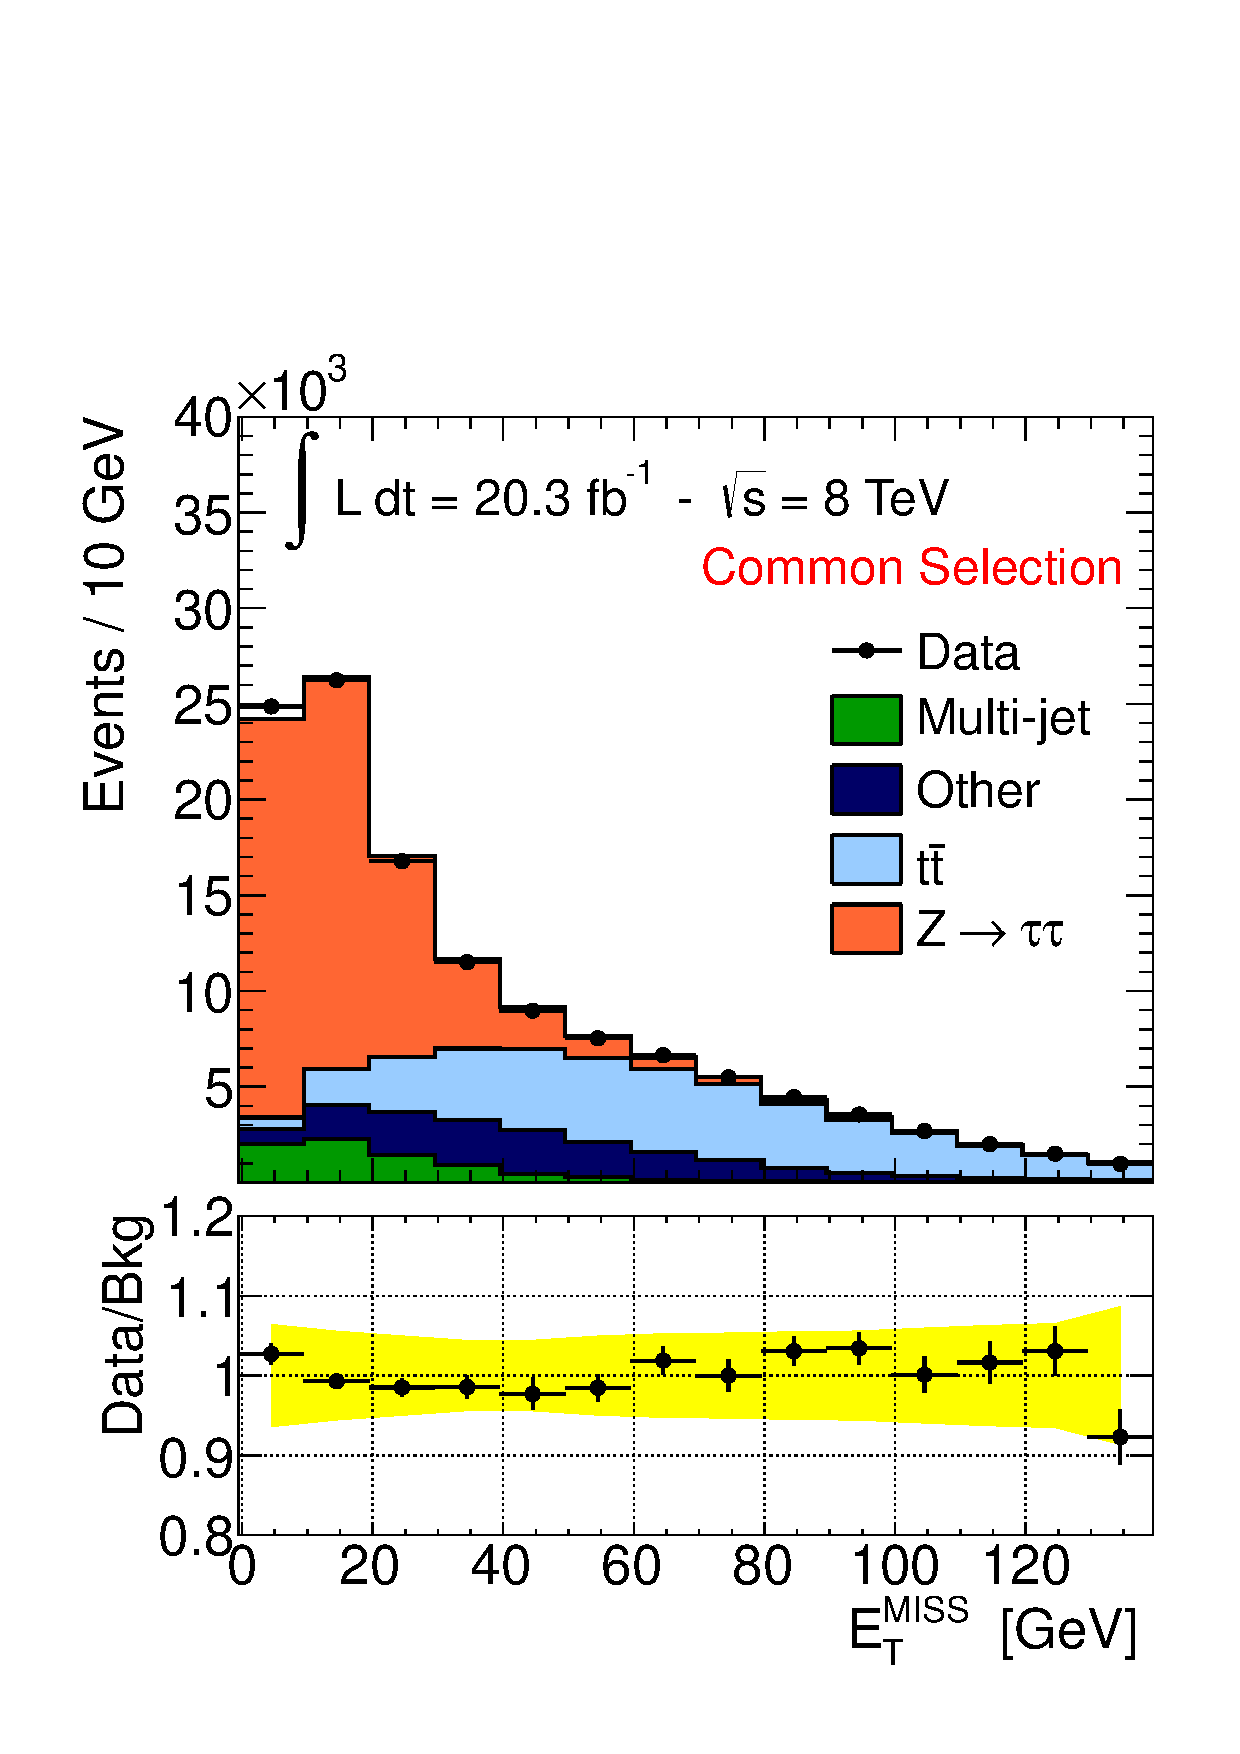
\includegraphics[width=0.47\textwidth]{figure/final_plots/std_presel_EtMiss.pdf}
            %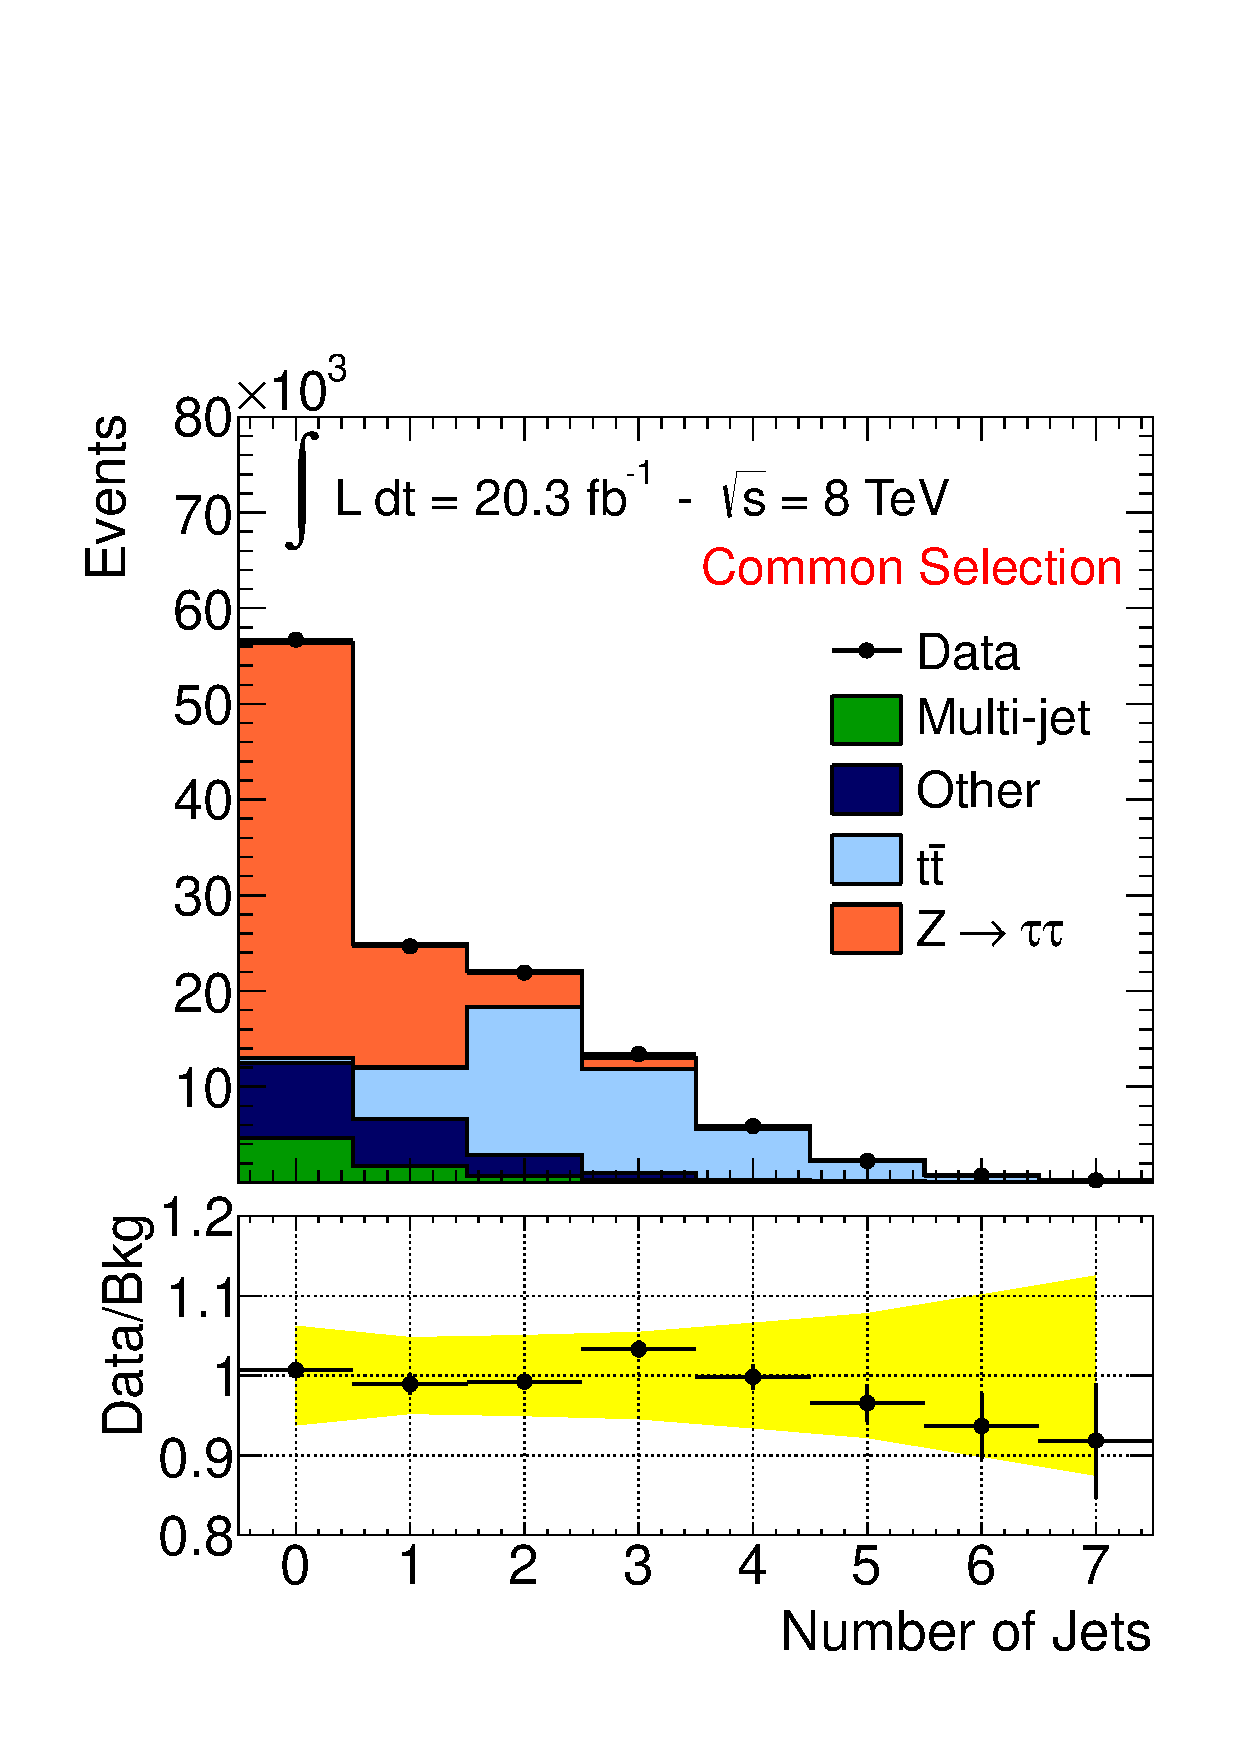
\includegraphics[width=0.47\textwidth]{figure/final_plots/std_presel_nJet_tag.pdf}
            \includegraphics[page=9,width=0.47\textwidth]{figure/final_plots/presel_total_final.pdf}
            \includegraphics[page=10,width=0.47\textwidth]{figure/final_plots/presel_total_final.pdf}
            \includegraphics[page=8,width=0.47\textwidth]{figure/final_plots/presel_total_final.pdf}
            \includegraphics[page=7,width=0.47\textwidth]{figure/final_plots/presel_total_final.pdf}


    \end{center}
    \caption{ 
	Observed and expected distributions of  kinematical variables after the common selection. 
	The predictions of the  background model are compared to  data (as in Figure~\ref{fig:selections}).}
   \label{fig:validation}
\end{figure}



\subsection{Validation of the \ttbar Background Simulation}
\label{sec:top_est}

The background contribution from top quark pair production is estimated using the POWHEG-PYTHIA Monte Carlo
generator. Since this is one of the major background processes for this analysis, a careful validation 
of the predicted contribution is needed. For this purpose a
signal-depleted data sample is enriched with \ttbar events  by requiring the presence of exactly two b-tagged jets after 
 the common selection criteria.
%Since this is one of the major backgrounds for this analysis (especially in b-tag category)
%a careful validation of this background model is need, for this purpose a  top quark enriched control region (CR)  
%is defined by adding to the preselection the further requirement of exactly two b-tagged jets in the event. 
Figures~\ref{fig:kinematicsttbar} and~\ref{fig:cutsttbar} show the distributions  of kinematical variables and of the
 discriminating variables for this  data sample. Good agreement between data and Monte Carlo prediction is found with 
%and shows that our top-quark background model describes well the data
%Also the prediction of the event yield in this CR is in good agreement with data: 
a ratio of  observed to predicted numbers of \ttbar events of $0.998 \pm 0.011\mathrm{(stat.)} \pm 0.110 \mathrm{(sys.)}\,.$
The total systematic uncertainty in the ratio is dominated by the uncertainty in the b-tagging efficiency. 
%In addition, this result could be used
%as a measure of $t\bar{t}$ normalisation avoiding systematic uncertainty on the theoretical cross section of
%this process. In this case, however, additional acceptance systematics would need to be evaluated in a dedicated study.
%
%with a dedicated RIVET analysis and uncertainties of the order of the cross section 
%uncertainty are expected, we then drop this possibility considering that wont bring  
%significant improvements.




\begin{figure}[tp]
     \begin{center}

        \subfigure[]{%MMC
            %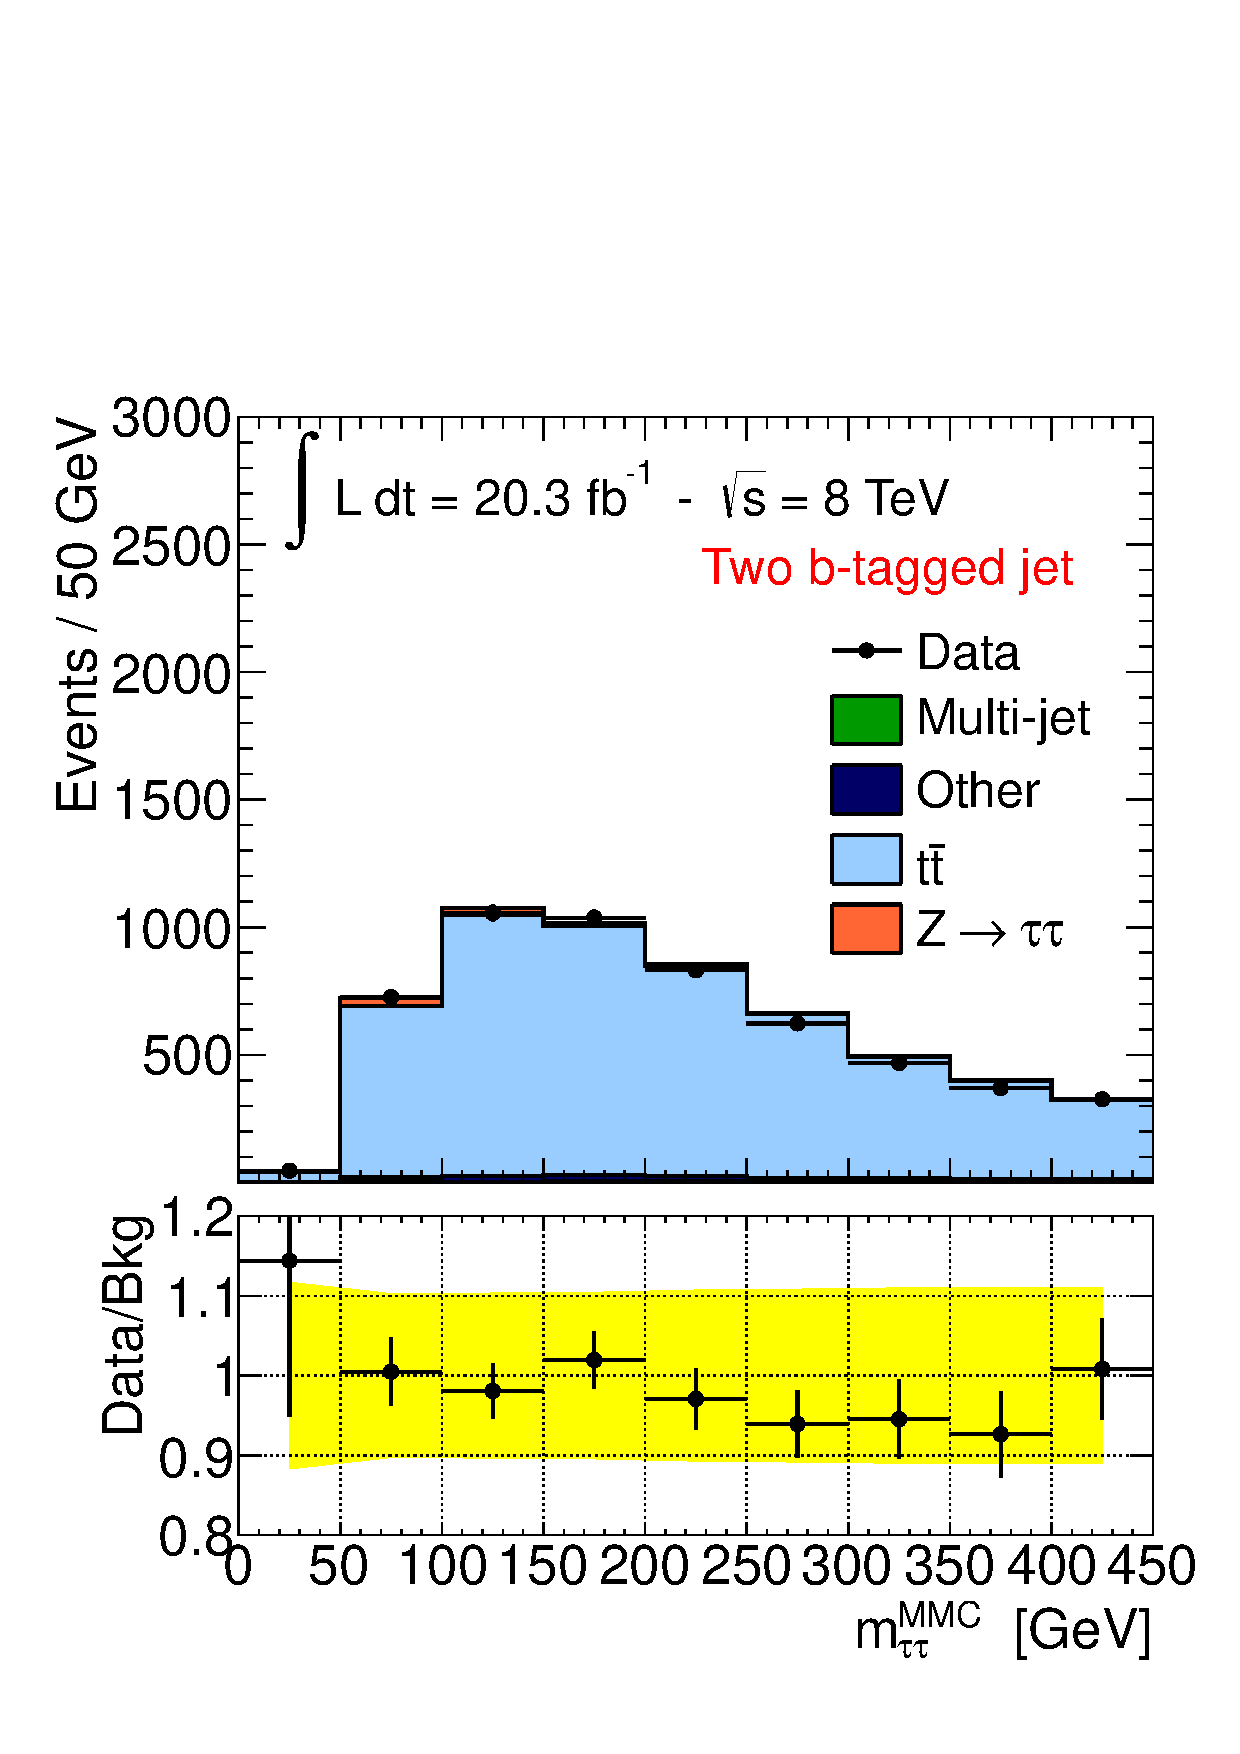
\includegraphics[width=0.47\textwidth]{figure/final_plots/std_presel_TwoBtag_mmc_mass.pdf}
            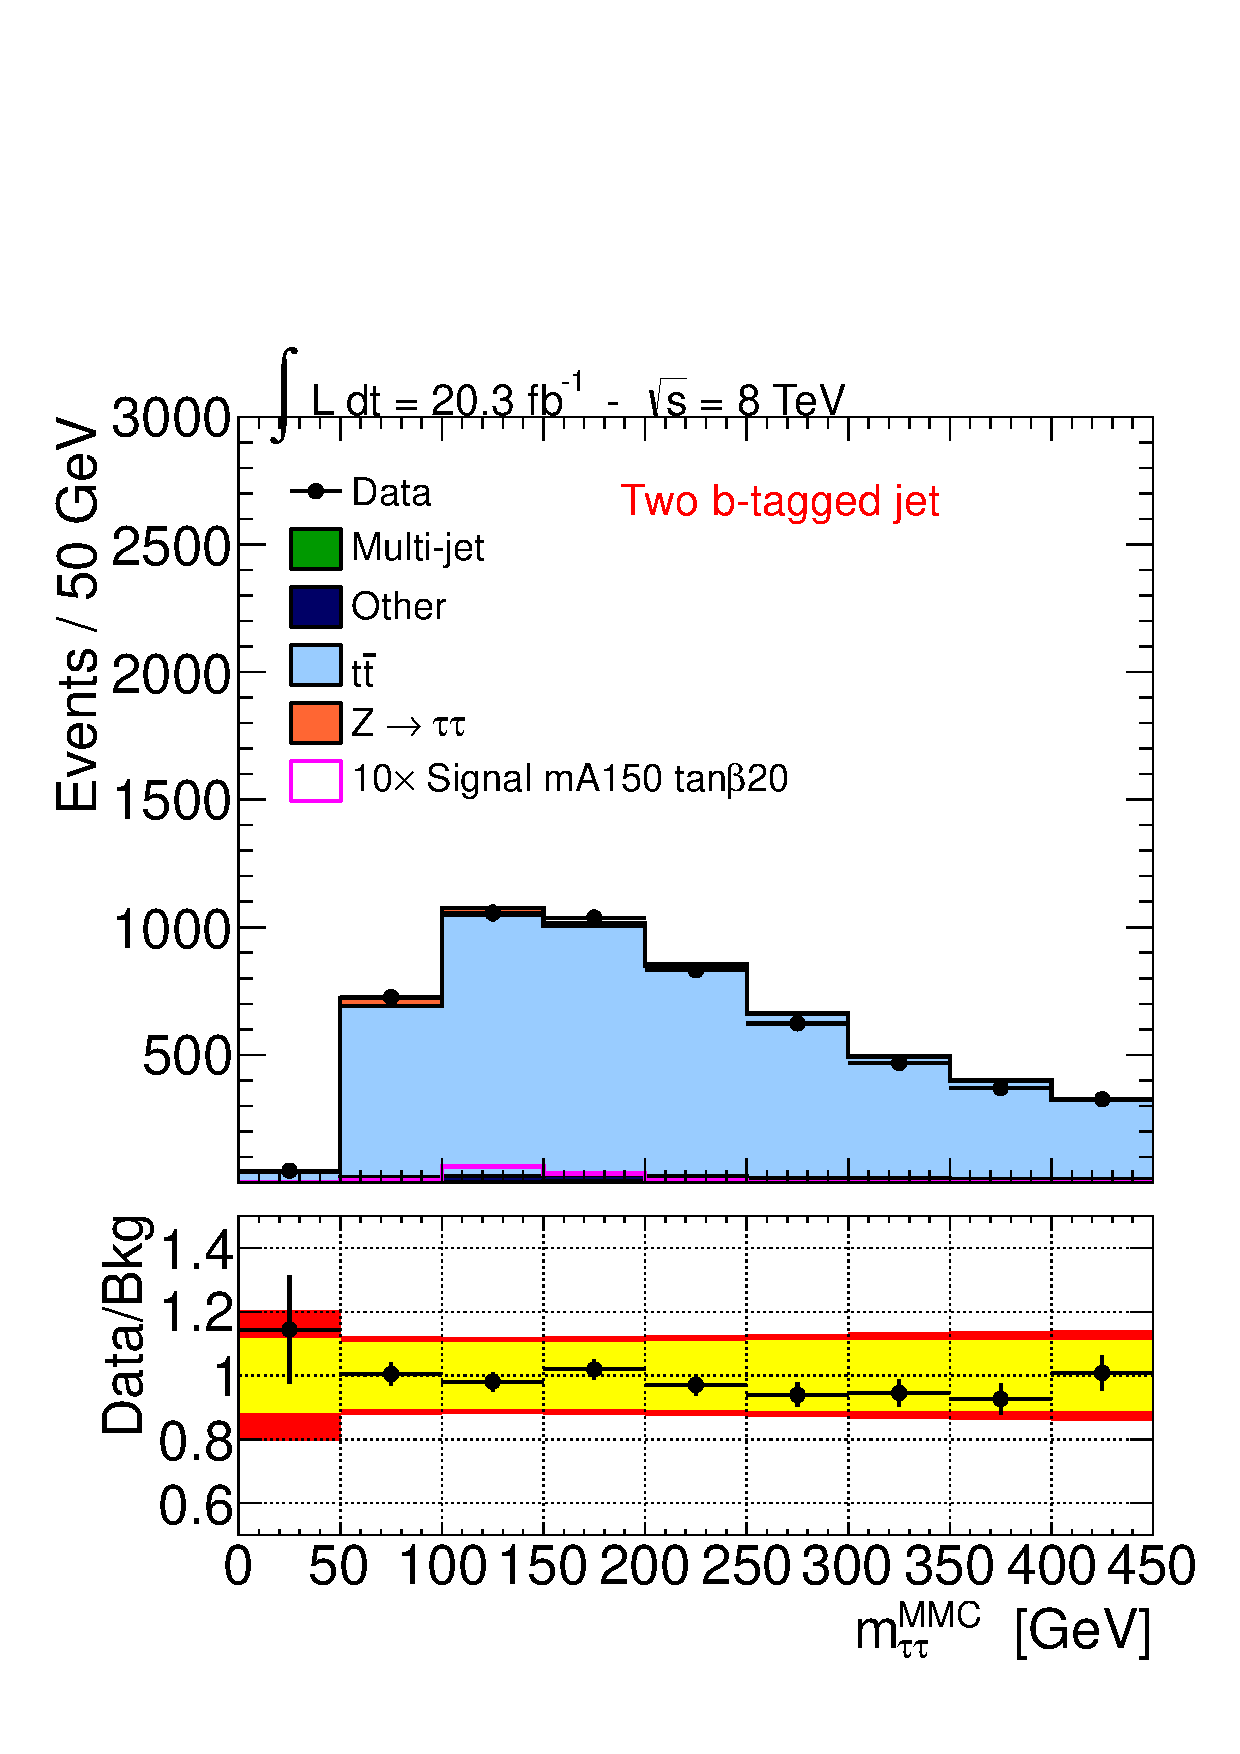
\includegraphics[page=1,width=0.47\textwidth]{figure/final_plots/twobtag.pdf}
        }
        \subfigure[]{%ele pT
           %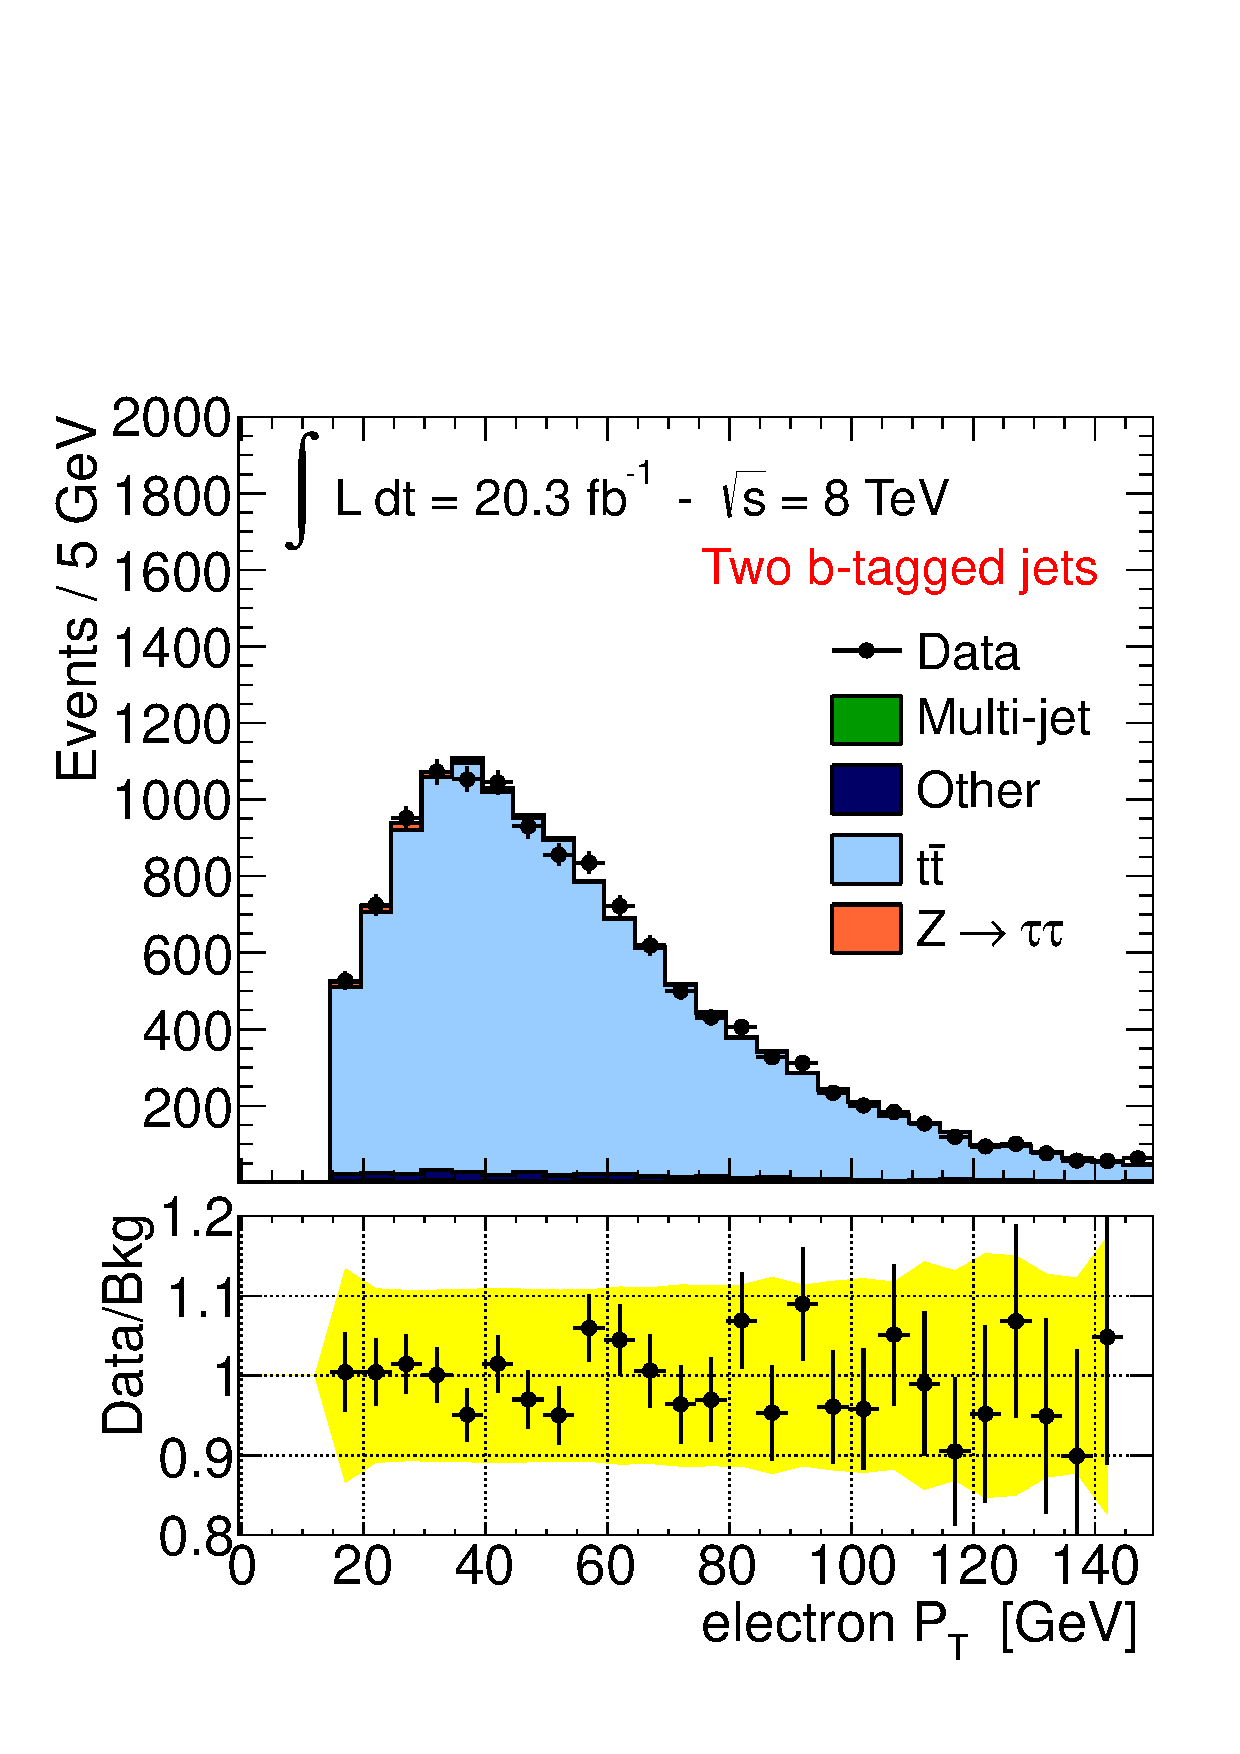
\includegraphics[width=0.47\textwidth]{figure/final_plots/two_btag_presel_TwoBtag_ele_pt.pdf}
            \includegraphics[page=7,width=0.47\textwidth]{figure/final_plots/twobtag.pdf}
        } 
        \subfigure[]{%Muon pt
            %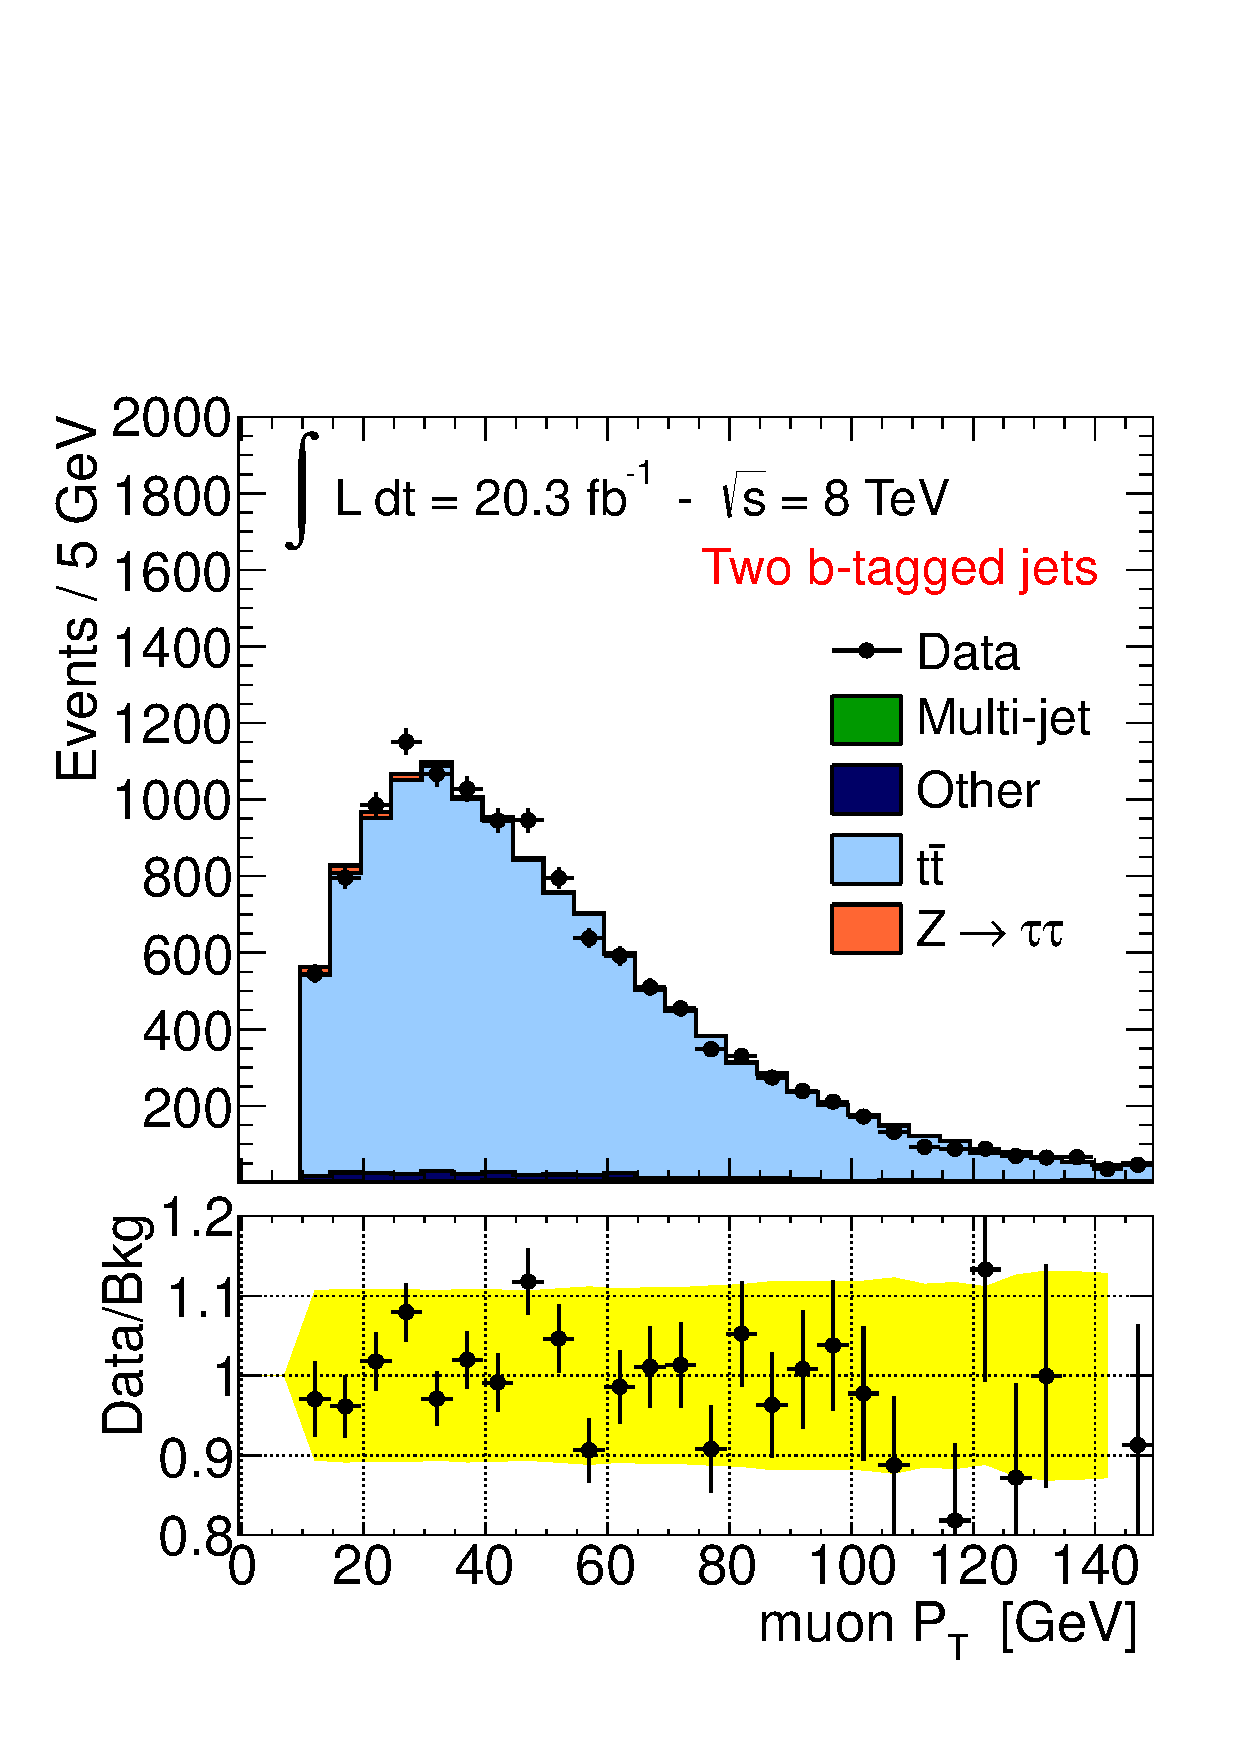
\includegraphics[width=0.47\textwidth]{figure/final_plots/two_btag_presel_TwoBtag_muon_pt.pdf}
            \includegraphics[page=6,width=0.47\textwidth]{figure/final_plots/twobtag.pdf}
        }
        \subfigure[]{%Muon pt
            %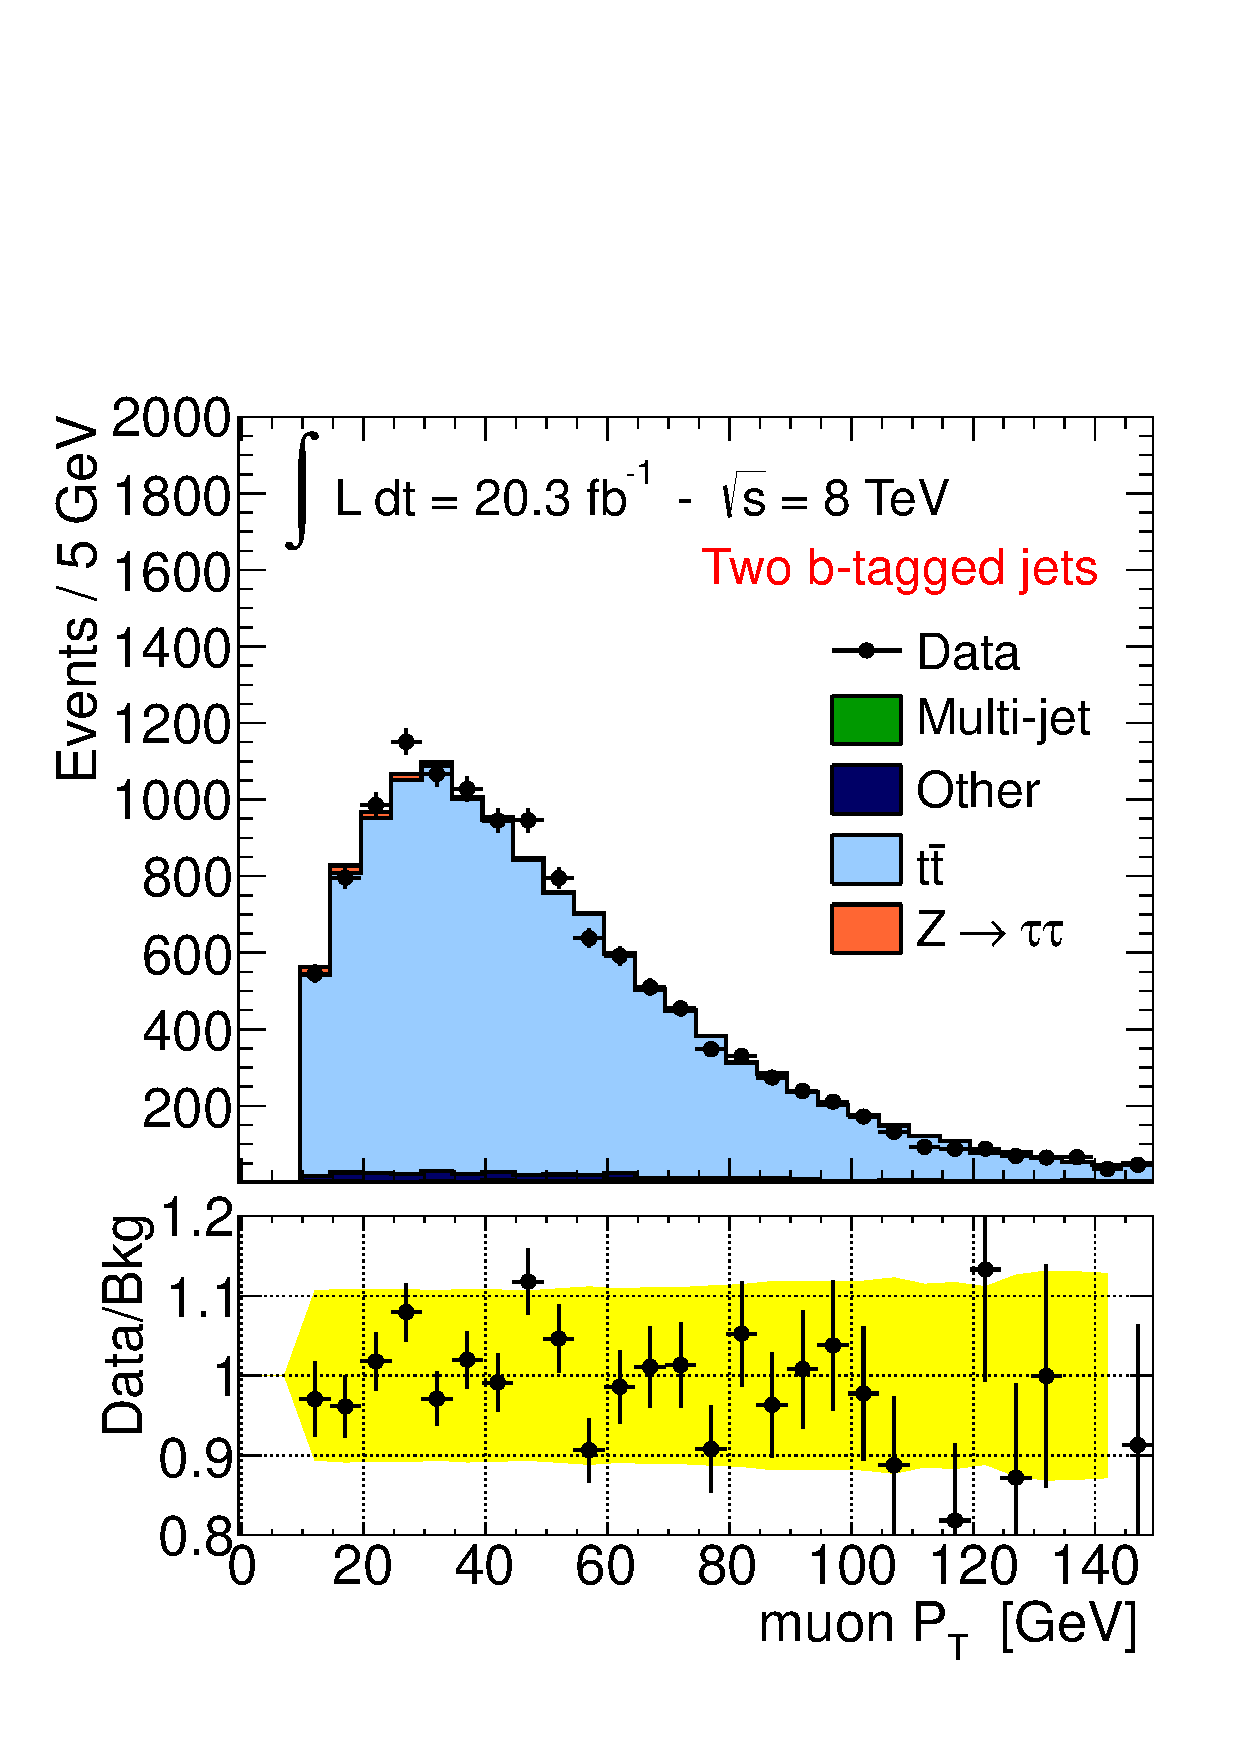
\includegraphics[width=0.47\textwidth]{figure/final_plots/two_btag_presel_TwoBtag_muon_pt.pdf}
            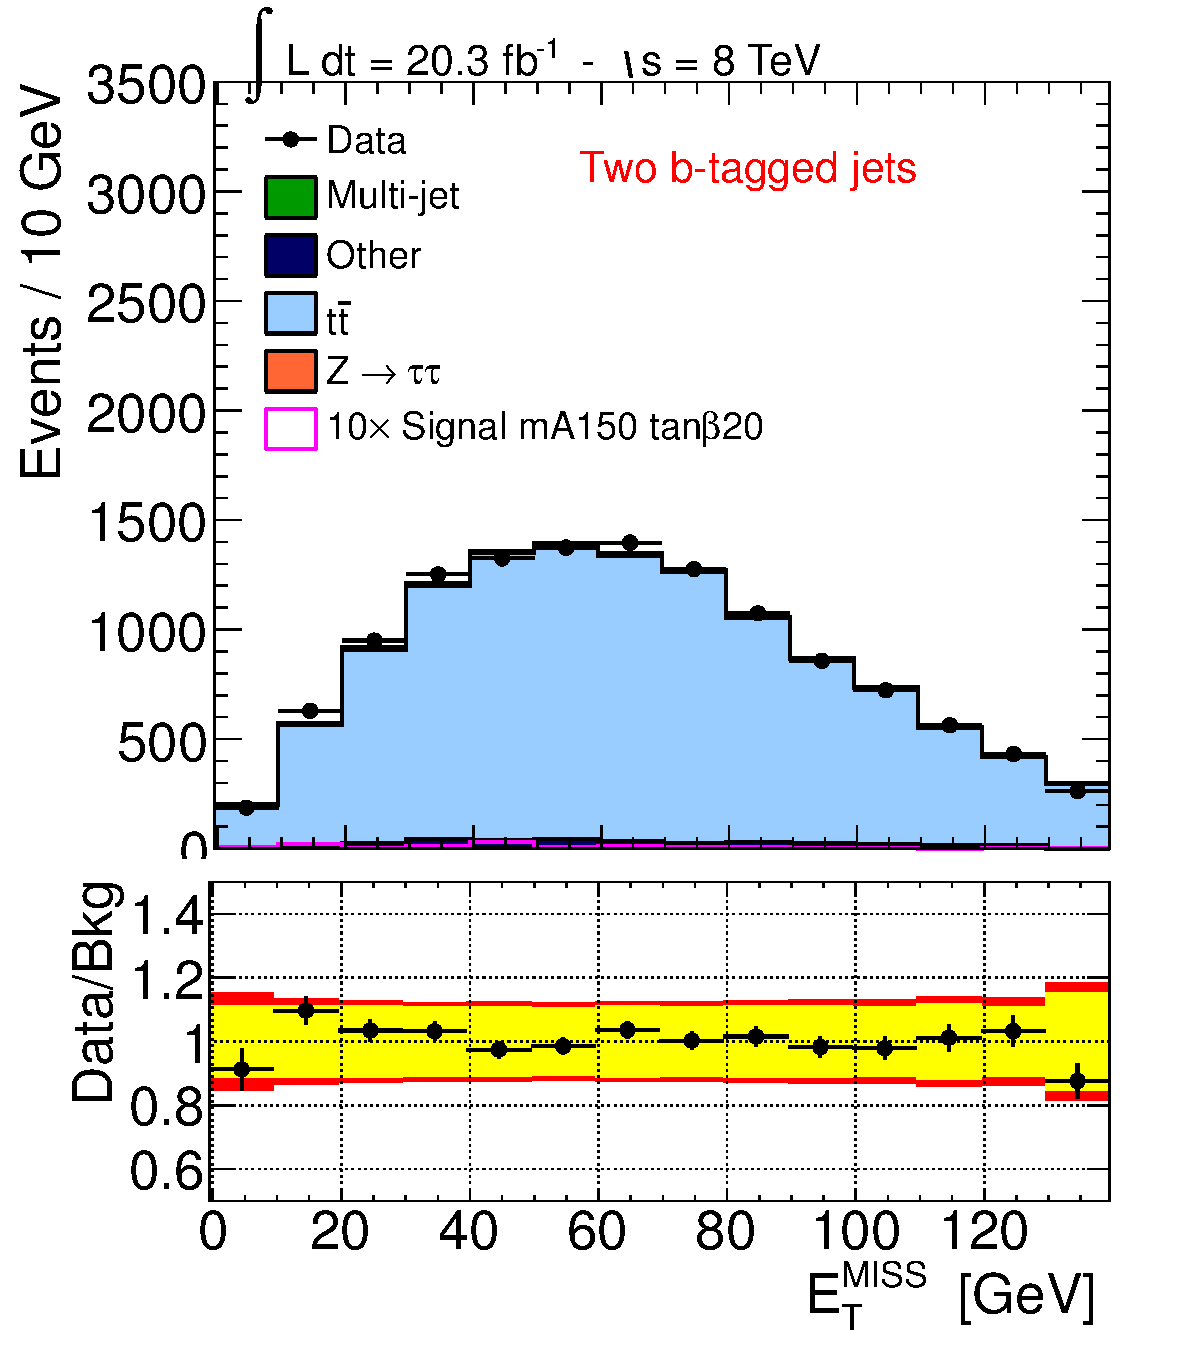
\includegraphics[width=0.47\textwidth]{figure/final_plots/etmiss_twobtag.pdf}
        }

    \end{center}
    \caption{ Observed and expected distributions  in the \ttbar validation sample of (a) the di-$\tau$ invariant mass estimated with $\mmc$, 
	(b) the electron and (c) the muon transverse momentum, (d) the missing transverse energy $\met$.
	The predictions of the  background model are compared to  data (as in Figure~\ref{fig:selections}).} 
   \label{fig:kinematicsttbar}
\end{figure}


\begin{figure}[htp]
     \begin{center}

        \subfigure[]{
            \label{fig:cuts_a} %DPhi
            %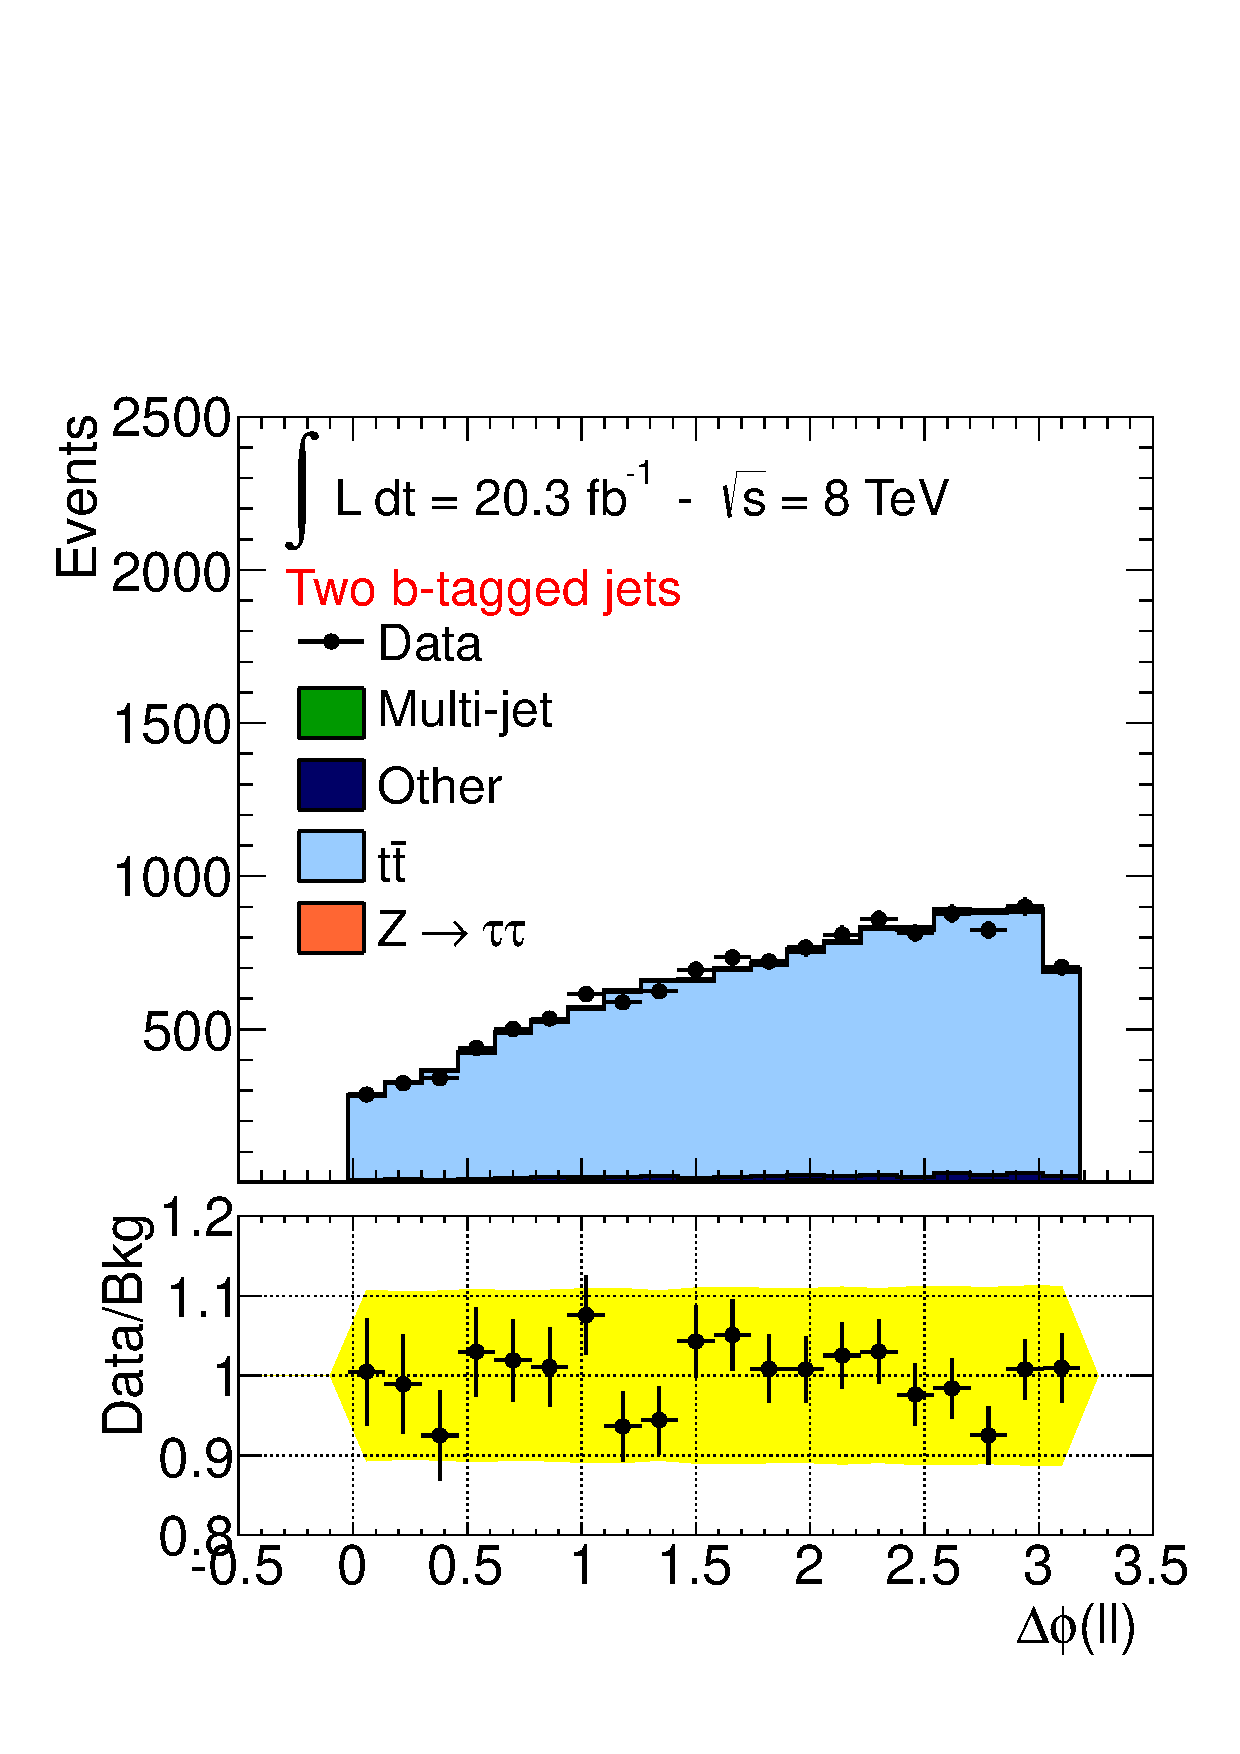
\includegraphics[width=0.47\textwidth]{figure/final_plots/two_btag_presel_TwoBtag_deltaPhi.pdf}
            \includegraphics[page=2,width=0.47\textwidth]{figure/final_plots/twobtag.pdf}
        }
        \subfigure[]{%CosDphi
            \label{fig:cuts_b}
            %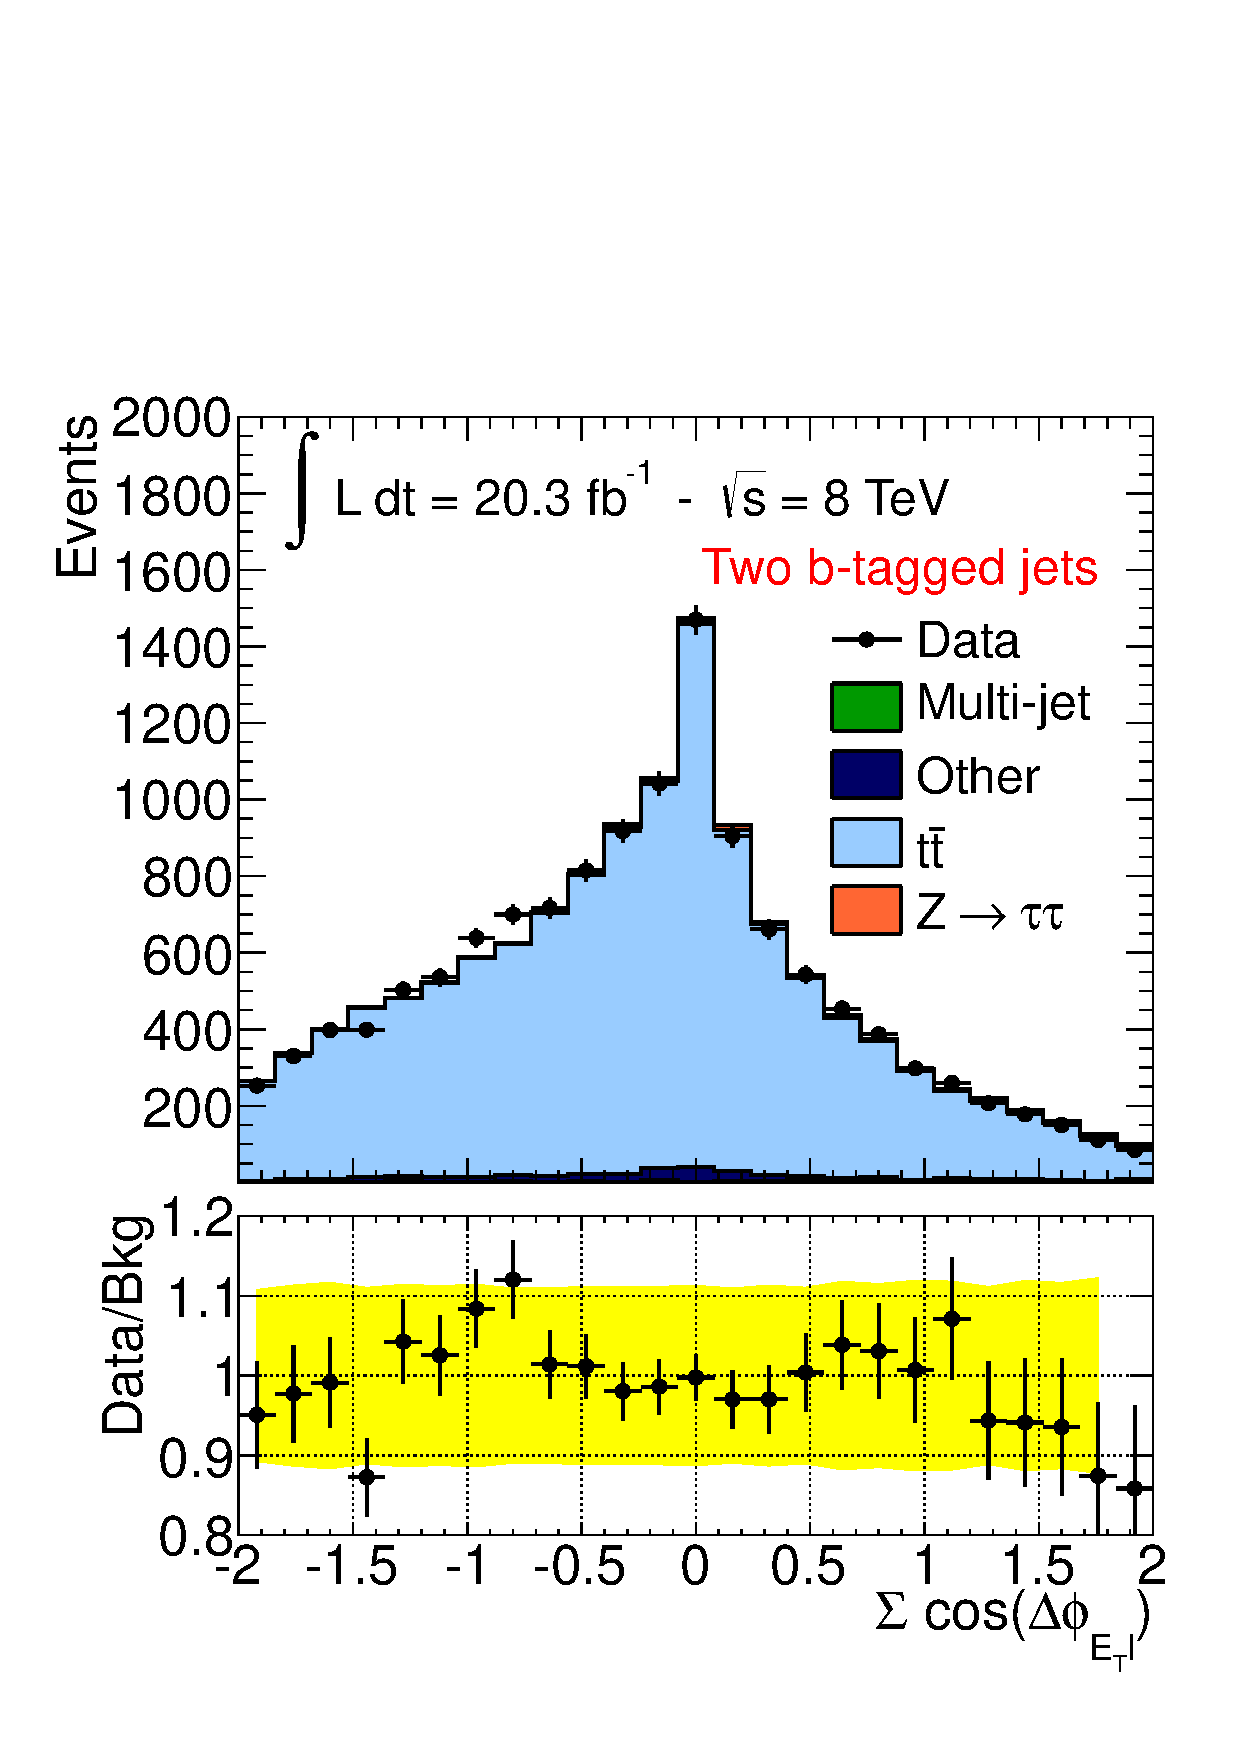
\includegraphics[width=0.47\textwidth]{figure/final_plots/two_btag_presel_TwoBtag_sum_cos_deltaPhi.pdf}
            \includegraphics[page=3,width=0.47\textwidth]{figure/final_plots/twobtag.pdf}
        }\\
        \subfigure[]{%Ht
            \label{fig:cuts_c}
            %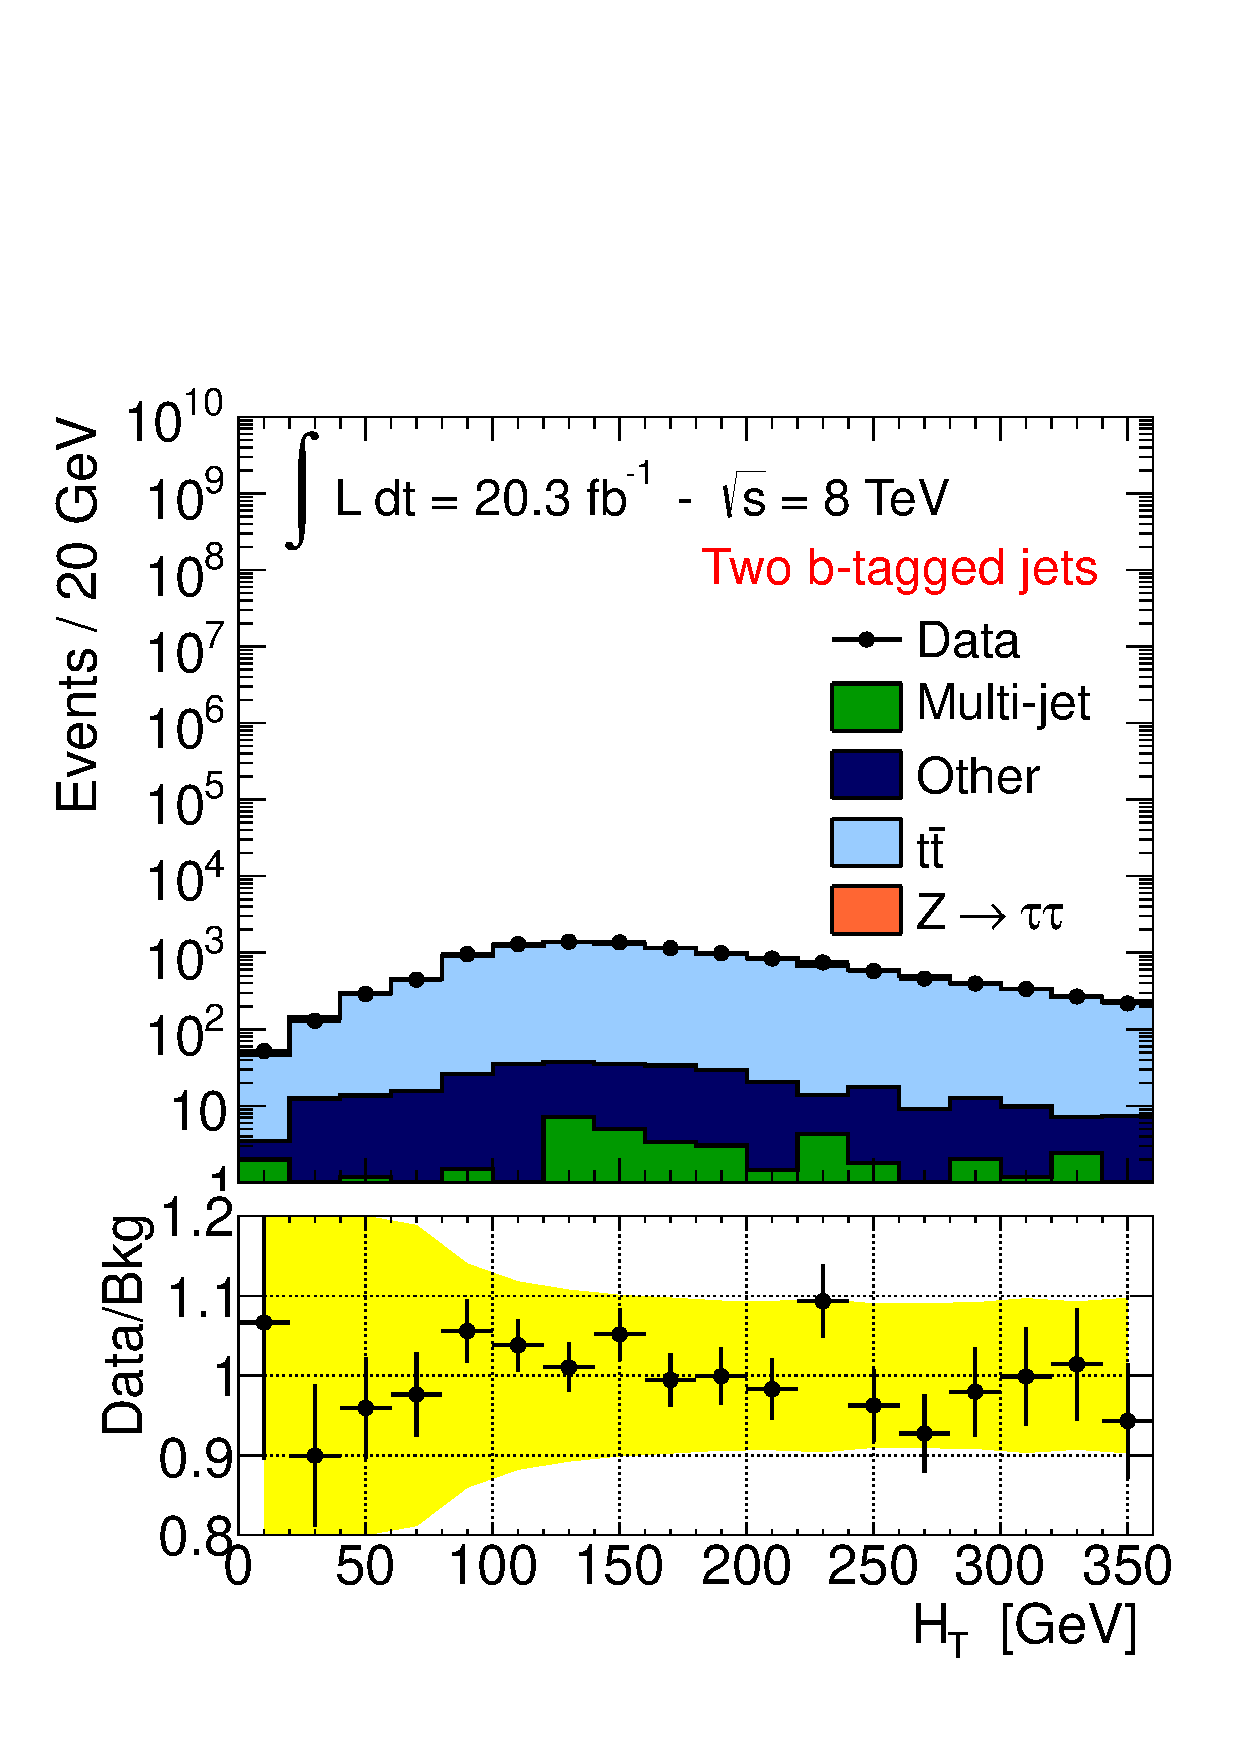
\includegraphics[width=0.47\textwidth]{figure/final_plots/two_btag_presel_TwoBtag_Ht.pdf}
            \includegraphics[page=4,width=0.47\textwidth]{figure/final_plots/twobtag.pdf}
        }
        \subfigure[]{%Lep+Et
            \label{fig:cuts_d}
            %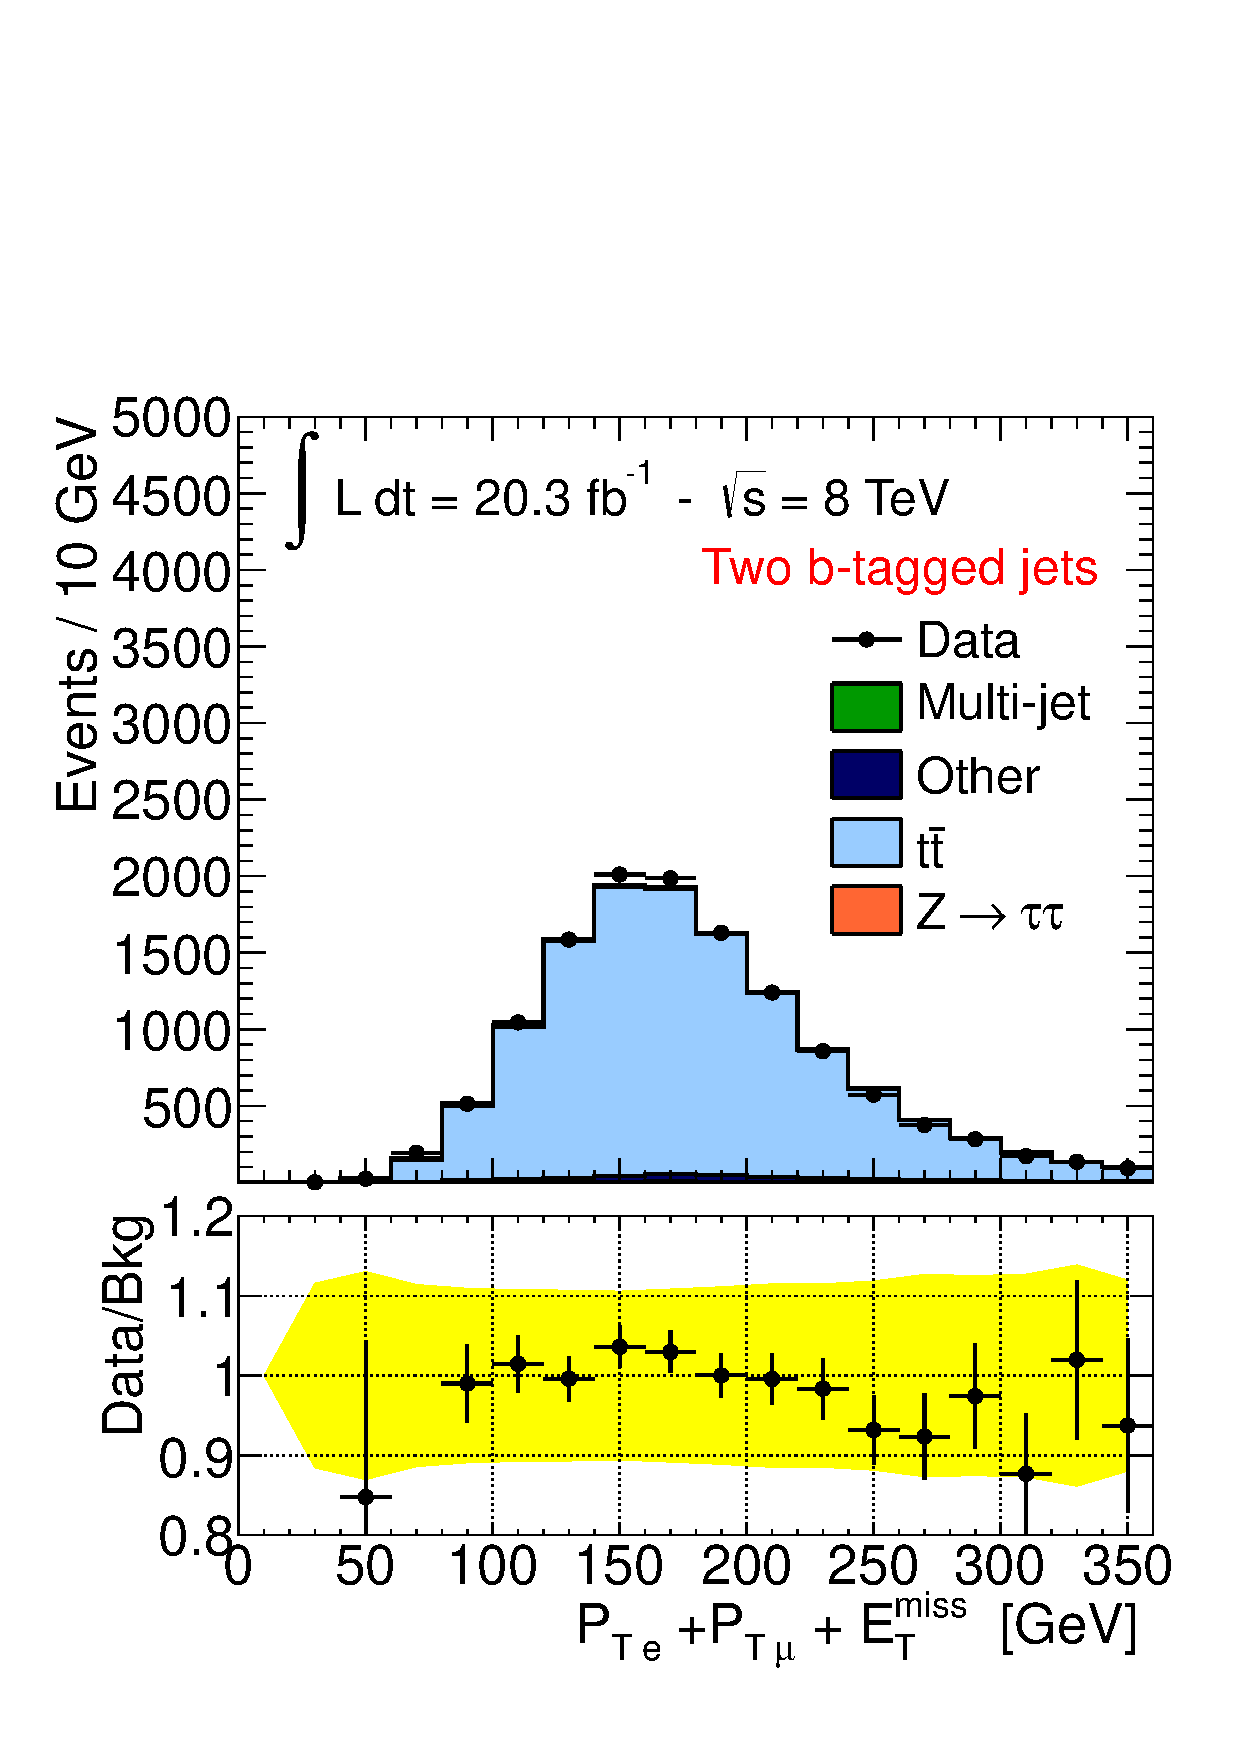
\includegraphics[width=0.47\textwidth]{figure/final_plots/two_btag_presel_TwoBtag_Et_plus_leptonPt.pdf}
            \includegraphics[page=5,width=0.47\textwidth]{figure/final_plots/twobtag.pdf}
        }

    \end{center}
    \caption{ Observed and expected distributions of the discriminating variables (a) $\Delta\phi(e-\mu)$,
      (b) $\sum\cos\Delta\phi$, (c) \SumLtMET and (d) \Ht  in the \ttbar validation sample.
	The predictions of the  background model are compared to  data (as in Figure~\ref{fig:selections}).}
 
   \label{fig:cutsttbar}
\end{figure}




\subsection{Measurement of Multi-jet Background}
\label{sec:qcd}


QCD multi-jet production represents an important background, 
especially in the b-vetoed event category, due to its high cross-section and the 
relatively low lepton \pt threshold  used in this analysis. The contribution of this
background is evaluated by the so-called ABCD data-driven technique.
In the ABCD method, the  data events after the common selection are split into four sub-samples: the
signal sample (A) defined by the event selection criteria described in Section~\ref{sec:selection}
and three signal-depleted control data samples (B,C,D) which are mutually exclusive  and 
enriched in multi-jet events. The three control data samples are defined by inverting the requirements on the relative 
sign of the electron and muon charge  and  on the isolation criteria. 
Both the calorimetric and tracking isolation criteria described in Section~\ref{sec:presel}  are inverted for  electron and muon 
with respect to the nominal values, thus defining the so-called non-isolated leptons. 
The data are divided into four samples of events with leptons of opposite sign charge (OS) 
or same sign charge (SS) and respectively isolated or non-isolated, as summarised in Table~\ref{table:qcd}.

\begin{table} [!tp]
\caption{Control data samples for the measurement of the QCD multi-jet background. The samples are defined by requirements on the relative
	sign of the two lepton charges (OS,SS) and on the lepton isolation  (isolated or non-isolated). See text.}
\centering
\begin{tabular}{c c c }
\hline
Data sample & Relative lepton charge & Lepton isolation \\ [0.5ex]
\hline
A (signal sample) & OS & isolated \\
\hline
B & SS & isolated \\
C & OS & non-isolated \\
D & SS & non-isolated \\ [1ex]
\hline
\end{tabular}
\label{table:qcd}
\end{table}


The ABCD method assumes that there is no correlation between the requirements of relative 
charge sign and of lepton isolation in QCD multi-jet events. In this case, the number $N_{A}$ of QCD multi-jet events in the signal sample $A$ 
can be estimated from the yields $N_B$, $N_C$ and $N_D$  of multi-jet events in the control samples $B$, $C$ and $D$ using the equation
\begin{equation} \label{eqn:qcdest}
N_{A}  = N_{B} \times \frac{N_{C}}{N_{D}} =  N_{B} \times \rqcd \,.
\end{equation}
%Here is  assumed that the events in the control samples come solely from QCD multi-jet processes, contamination
%from electroweak (W and Z + jets, dibosons) and top processes
%($t\bar{t}$ and single top production) are  subtracted in each control sample 
%using the MC prediction for their event yield.  
To obtain the  QCD multi-jet event yields in the control data samples, the contributions of
contaminating electroweak (W+jets, Z+jets and dibosons) and top quark 
($t\bar{t}$,  single top quark production) processes are  subtracted based on the prediction from simulation.
Tables~\ref{table:qcd_yield_bveto}~and~\ref{table:qcd_yield_btag}
show the observed event yields in the control samples at different stages of the event selection along with the
non-QCD background predictions  which are subtracted.
Contamination by signal events has been evaluated in all  three control samples for different  $m_{A}$ and $\tan\beta$ values in the
range considered in this analysis. The highest signal contamination of 0.2\% is observed\footnote{
This signal contamination originates mainly from the production in association with b-quarks and,
as it scales with the cross section, it is an order of magnitude smaller for $\tan\beta = 20\,.$
} in sample B for $m_{A} = 300$ GeV and $\tan\beta = 50$.

\begin{table} [!p]
	\caption{Numbers of observed events and the  non-QCD contributions at different stages of the event selection for the b-vetoed category. 
	The error on  \rqcd ratio is statistical only.}
\begin{small}
	\begin{tabular}[c]{l r c c c c}
%%%%%%%%%%%%%%%%%%%%%%%%%%%%%%%%%%%%%%%%%%%%%%%%%%%%%%%
\hline
\hline 
Event Selection  &  		& B & C & D &  \rqcd \\ 
\hline
Common Selection 	&   Data	&6189			&604628			&312901		    &	1.929 $\pm$  	0.004		\\
	        &   non-QCD	&2510 $\pm$  180  	&1090 $\pm$   30  	&730	$\pm$ 35    &				\\
\hline
B-veto	     	&   Data	&5673		  & 558217 		& 284847		    &	1.960	$\pm$	0.004	\\
	     	&   non-QCD	&2220	$\pm$ 180 & 710 $\pm$ 30	& 415 $\pm$	30	    &				\\
\hline
$\Delta\phi_{e,\mu}$  &   Data		&4610		&532583 		&271404		    	    &	1.962	$\pm$	0.005	\\
	     &   non-QCD	&1700 $\pm$170	&580 $\pm$	30	& 345 $\pm$	30	    &				\\
\hline
$\sum\cos\Delta\phi$ &   Data& 3417	&486747 		& 247712	   		    &	1.965	$\pm$	0.005 	\\
	     &   non-QCD     & 1120  $\pm$ 100	& 370 $\pm$ 	20		& 230 $\pm$	20  &				\\
\hline
$\mmc > 0.$    &  Data		& 3177		& 479967 		& 244276	    	    &	1.965	$\pm$	0.005	\\
	     &   non-QCD	& 1000 $\pm$ 100	& 300  $\pm$ 17		&190	$\pm$ 20    &			\\[1ex]
\hline
\hline
%%%%%%%%%%%%%%%%%%%%%%%%%%%%%%%%%%%%%%%%%%%%%%%%%%%%%%%
	\end{tabular}
\end{small}
	\centering
	\label{table:qcd_yield_bveto}
\end{table}

\begin{table} [!p]
	\caption{Numbers of observed events and the  non-QCD contributions at different stages of the event selection for the b-tagged category. 
	The error on  \rqcd ratio is statistical only.}
\begin{small}
	\begin{tabular}[c]{l r c c c c}
%%%%%%%%%%%%%%%%%%%%%%%%%%%%%%%%%%%%%%%%%%%%%%%%%%%%%%
\hline 
\hline 
Event Selection  &  		& B & C  & D &  \rqcd \\
\hline
Common Selection&   Data	&6189			&604628			&312901		    &	1.929 $\pm$  	0.004		\\
	        &   non-QCD	&2510 $\pm$  180  	&1090 $\pm$   30  	&730	$\pm$ 35    &				\\
\hline
B-tag	     	&   Data	&419		&44619 			&27257		    &	1.64	$\pm$	0.01	\\
	     	&   non-QCD	&215 $\pm$  10	&310 $\pm$	12	&277 	$\pm$ 13    &				\\
\hline
$\Delta\phi_{e,\mu}$  &   Data		&230		&38810 			&23316	    &	1.67	$\pm$	0.01	\\
	     &   non-QCD	&104 $\pm$ 6	&200 $\pm$	10	&175	$\pm$ 7	    &				\\
\hline
$\sum\cos\Delta\phi$ &   Data & 149		&31379 			&18779		    &	1.67	$\pm$	0.02	\\
	     &   non-QCD      & 67 $\pm$ 5	&127 $\pm$	8	&114 $\pm$	6   &				\\
\hline
$\sum H_T$ &   Data	      & 83		& 27781 		&15626		    &	1.78	$\pm$	0.02	\\
	&   non-QCD	      & 23 $\pm$  4	& 25 $\pm$	3	& 22 $\pm$   3	    &				\\ 
\hline
\SumLtMET &   Data	&71		&27735 	&15590		    &	1.78	$\pm$	0.02	\\
	     &   non-QCD	 & 10 $\pm$	3	& 22  $\pm$ 3		&18	$\pm$ 2	    &			\\
\hline
$\mmc > 0.$    &  Data	& 70	& 27634 	& 15522		    			    &	1.78	$\pm$	0.02	\\
	     &   non-QCD	& 9 $\pm$ 3	& 20  $\pm$ 3		&17	$\pm$ 2	    &			\\[1ex]
\hline
\hline
%%%%%%%%%%%%%%%%%%%%%%%%%%%%%%%%%%%%%%%%%%%%%%%%%%%%%%
	\end{tabular}
\end{small}
	\label{table:qcd_yield_btag}
\end{table}

\begin{figure}[!p]
	\begin{center}
	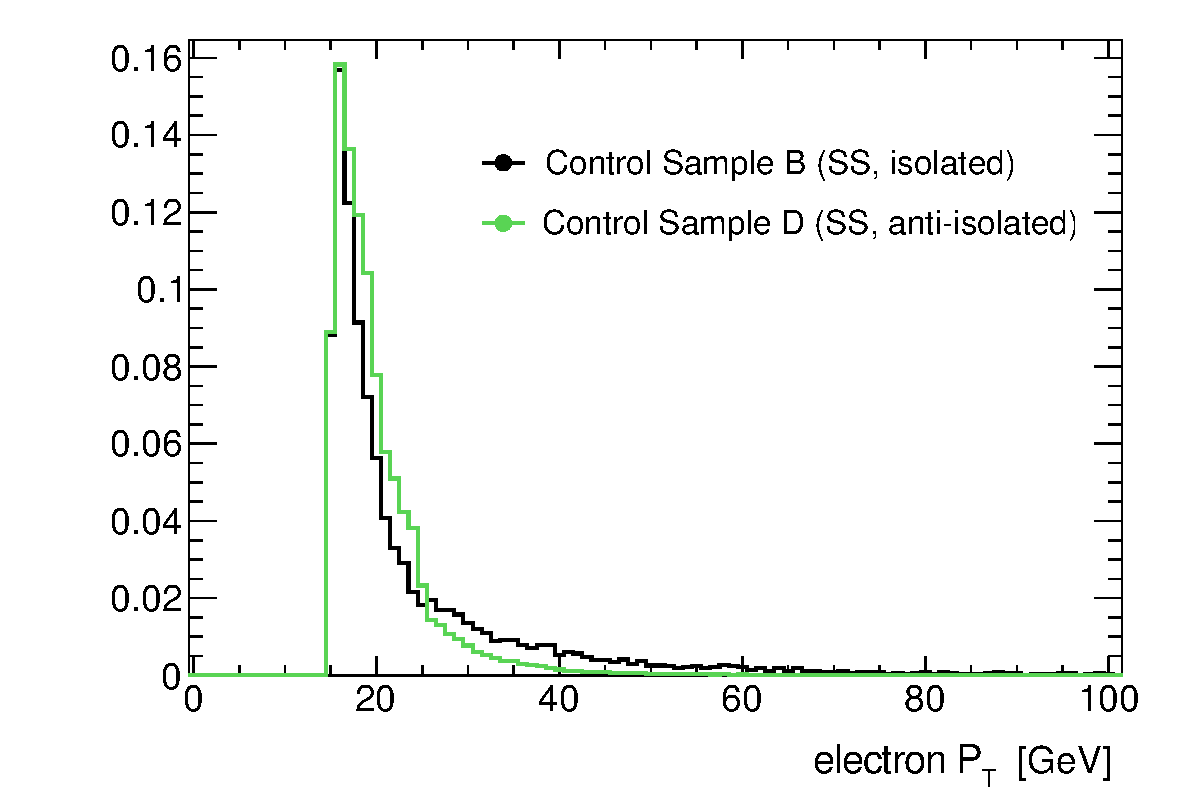
\includegraphics[width=9cm]{figure/ABCD_regionB_Vs_regionD2}
	\end{center}
	\caption{Comparison of the electron \pt~distributions in control samples B and D, showing the bias due to the trigger. 
	The histograms are normalised to the same area.}
	\label{fig:BvsD}
\end{figure}

\begin{figure}[p]
	\begin{center}
	     
%	\subfigure[]{
		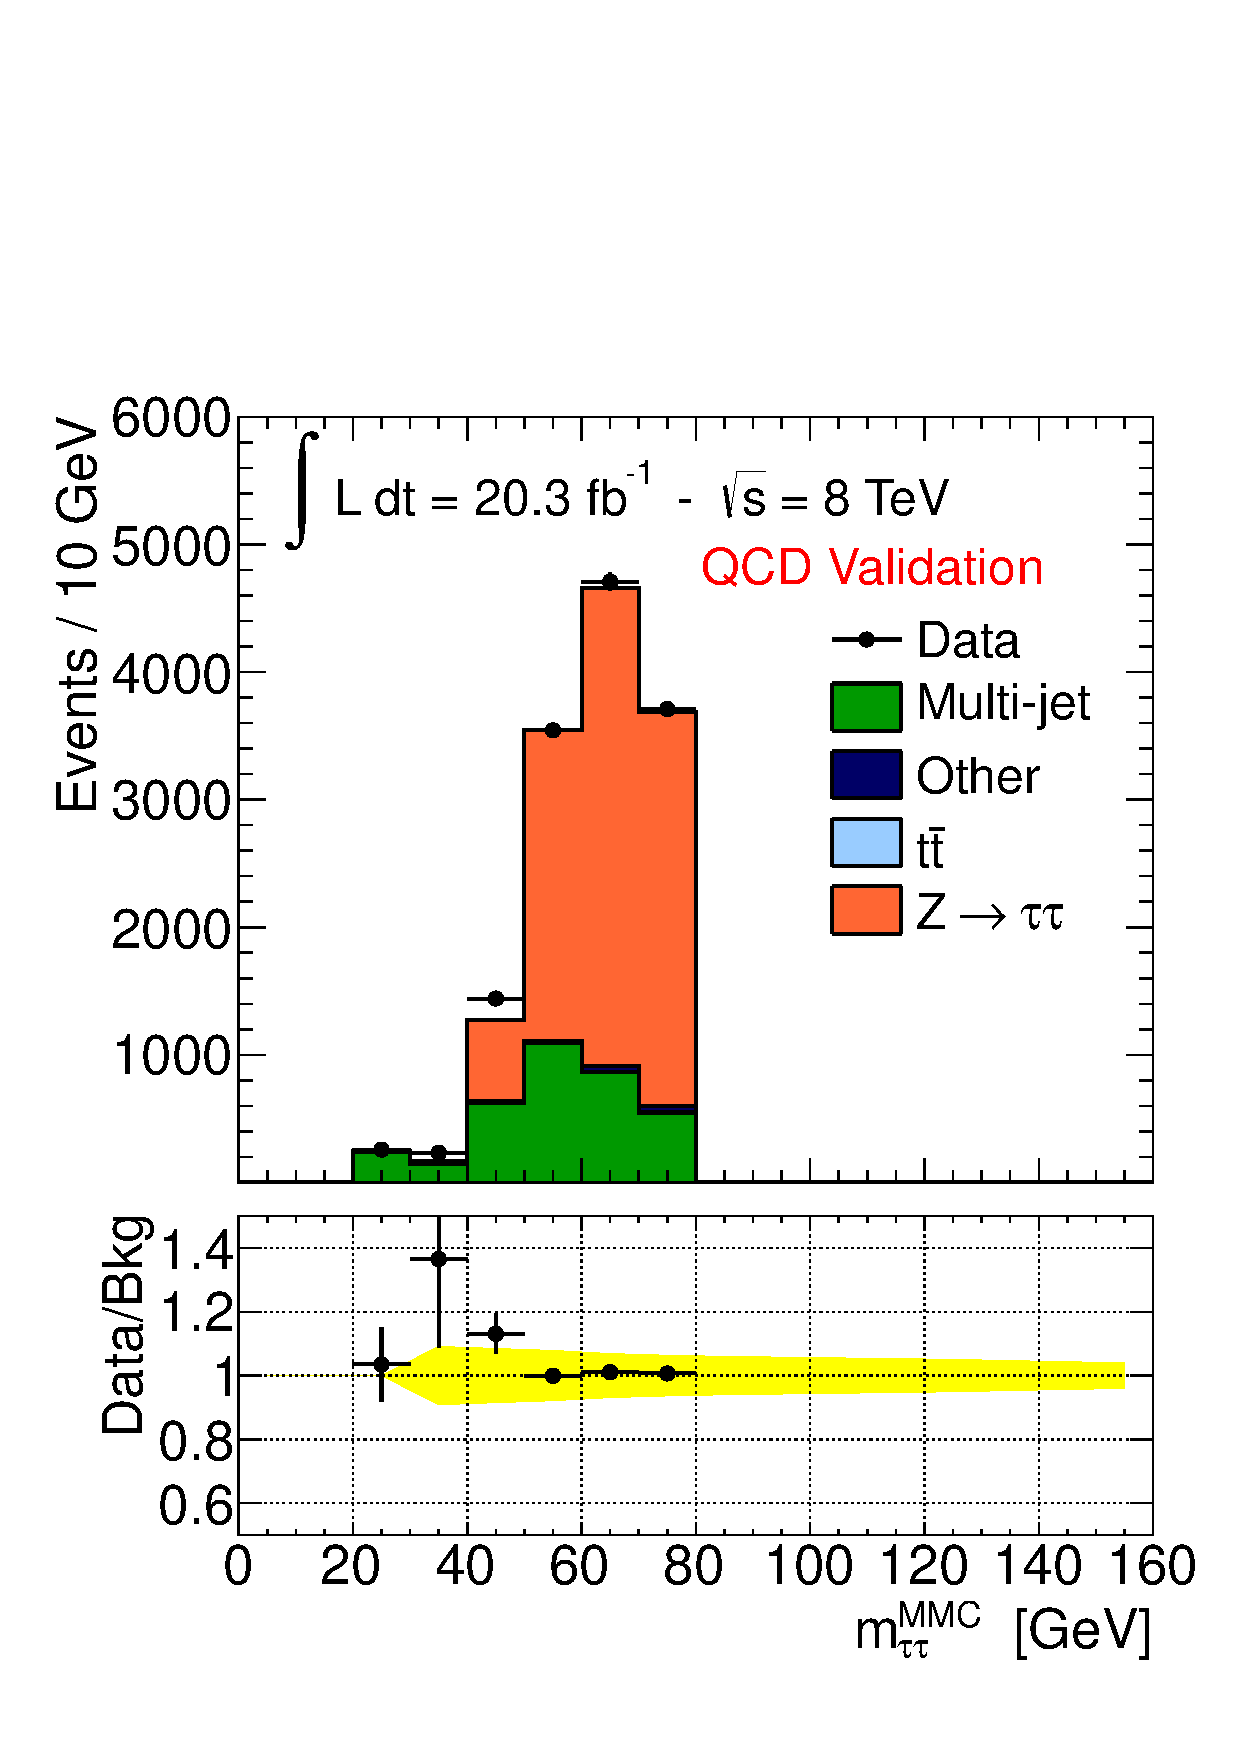
\includegraphics[width=0.44\textwidth]{figure/QCD/qcd_CR_emb_mmc_mass.pdf}
%	        }
%	\subfigure[]{
	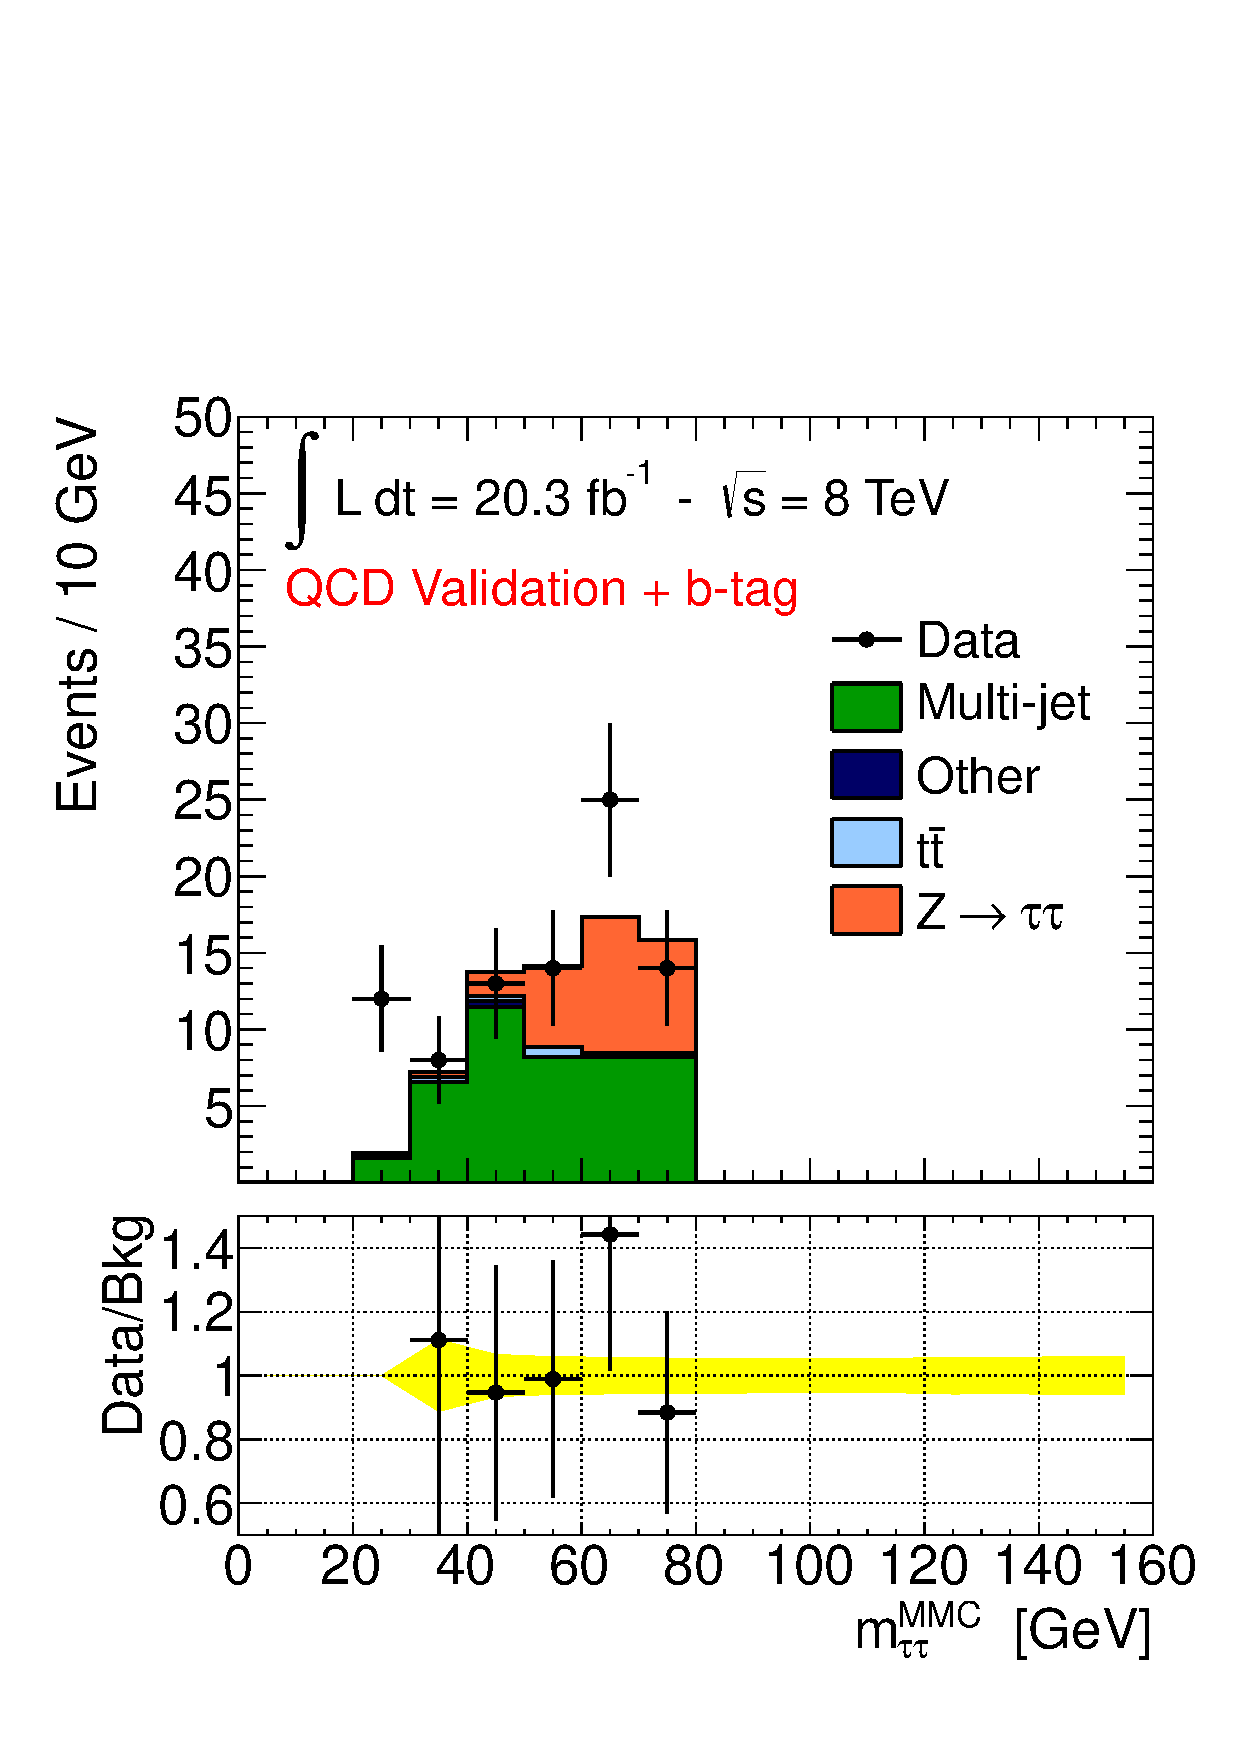
\includegraphics[ width=0.44\textwidth]{figure/QCD/qcd_CR_emb_Btag_mmc_mass.pdf}
%	}
	
	\end{center}
	\caption{ \mmc distributions for the QCD validation samples 
	defined in Section~\ref{sec:qcd} without~(left) and with~(right) additional requirement of exactly one b-tagged jet in the final state.
	The error bars and the yellow band indicate the statistical and systematic uncertainties, respectively.}
%	The prediction for the $\Ztt$ is obtained with the embedded sample, simulation is employed for all the other backgrounds (except QCD multi-jet).
%	The notation ``Other'' stands   for the electroweak processes $\Wlnu$, $\Zll$, diboson and single top quark production.
	\label{fig:ABCD_cr}
\end{figure}


The shapes of the kinematical distributions in QCD multi-jet events 
are modelled  by the data sample B which is expected to have similar kinematical properties as   the signal sample.
A drawback of this choice is a rather low number of events and a higher contamination with non-QCD process compared to samples C and D.
Sample B is chosen  to avoid  bias in the shapes due to the isolation requirements at the trigger level, since the single-electron trigger 
already imposes isolation requirements. 
%the trigger:  an isolated trigger is used 
%for electrons (as described in Section~\ref{sec:eventsel}), where the offline requirement equivalent to this trigger choice is $\ptcone20/\pt <0.1$.
Figure~\ref{fig:BvsD} shows the comparison of the electron $\pt$ distributions in samples B and D. In the latter, 
high-$\pt$ electrons are suppressed as they do not pass the trigger selection. 
The trigger isolation requirement could in principle also 
bias the ratio \rqcd. This possibility has been investigated 
in a dedicated study discussed in Appendix~\ref{appendix:qcd}.
To  good approximation, the  trigger effects cancel  in the ratio
\rqcd and no additional systematic uncertainty arises.




To test the predictions of the ABCD method,  an additional validation sample has been defined with the following criteria applied after
the common selection:
\begin{itemize}
\item \MET $< 20$ GeV,
\item \Ht $< 70$ GeV and \SumLtMET$ < 50$ GeV,
\item $0 < \mmc < 80$ GeV  .	 
\end{itemize}
These requirement are designed to enhance the multi-jet background contribution with respect to \Ztautau keeping the final 
state kinematics as similar as possible to the signal sample.
Figure~\ref{fig:ABCD_cr} shows the \mmc distribution for this validation sample with and without the  b-tagging requirements.
Agreement between data and the background predictions is found within statistical and detector-related systematics uncertainty. 

%%%%	this table is not that useful

%\begin{table} [p]
%	\caption{Contribution to the different control regions from non-QCD background, after the preselection. }
%	\centering
%	\begin{tabular}{ c c c c c c c}
%%%%%%%%%%%%%%%%%%%%%%%%%%%%%%%%%%%%%%%%%%%%%%%%%%%%%%%%
%\hline
%Region  &  \Ztautau	 & $t\bar{t}$	 & W + jets	 & $Z \rightarrow ll$ + jets & Single Top 	& Dibosons \\ [0.5ex]
%\hline
%  B 	& 341 	$\pm$ 6	&	700$\pm$ 11	&	3398$\pm$ 180	& 830 $\pm$ 58	     &	178$\pm$ 8 		&   612$\pm$ 10  \\
%  C 	& 16 	$\pm$ 2	&	719$\pm$ 12	&	409$\pm$ 50	& 17 $\pm$ 4	     &	103$\pm$ 6		& 13$\pm$ 1 \\
%  D 	& 8	$\pm$ 2	&	539$\pm$ 10	&	49$\pm$	12	& 24$\pm$  7	     &	67$\pm$	 4		& 6$\pm$ 1 \\[1ex]
%\hline
%%%%%%%%%%%%%%%%%%%%%%%%%%%%%%%%%%%%%%%%%%%%%%%%%%%%%%%
%	\end{tabular}
%	\label{table:qcd_mc}
%\end{table}


%%%%%%%%%%%%%%%%%%%%%%%%%%%%%%%%%%%%%%%%%% PUT FINAL NUMBERS!!!!!!!!!!!!!!!! %%%%%%%%%%%%%%%%%%






Systematic uncertainties are assigned on the scaling factor \rqcd and on the shape of
the discriminating variable \mmc to take into account any correlation between the isolation and the relative charge 
of the leptons as detailed in Section~\ref{sec:Systematics}.





\subsection{$Z \rightarrow \tau\tau$ + Jets Background Measurement}\label{sec:ztau}


The  \Ztautau production is the main  source of  background in this analysis and needs to be well understood.
Unfortunately, for a light Higgs boson, it is impossible to fully discriminate between  \Ztautau decays 
and the signal because of the similarity of the final state, a dedicated signal-free data control sample, thus, cannot be defined.
However, thanks to the small Higgs boson coupling to muons, \Zmumu events from data  provide a good starting point to 
model \Ztautau events. A hybrid approach relying on data and simulation known as  "embedding" is used for this purpose.
$\Zmumu$ event candidates are selected in data. Each of the two muons from the $Z$ decay is then substituted by the decay 
products from a simulated decay of a $\tau$ lepton, which has the same kinematical properties as the muon. 
The energy deposits in the calorimeters and the reconstructed tracks within a cone  around the muon are subtracted in the data
and substituted by the simulated $\tau$ lepton decay.  Further details on the embedding technique can be found in \cite{Embedding, SMold}.

%The selection of the \Zmumu input data requires exactly two combined, opposite charged
%muons, where the leading muon has a transverse momentum $\pt > 20 \GeV$ and 
%the sub-leading muon $\pt > 15\GeV$. Both muons are requited to lie within $|\eta|<2.5$ and to be isolated with 
%$\ptcone 20/\pt<0.2$ (see Section~\ref{sec:presel}). Additionally 
%the invariant mass of the two muons is required to be in the range $M_{\mu\mu} > 40$ GeV.
%Once the muon pair events are selected, all tracks and calorimeter cells associated to the muons are 
%removed from the \Zmumu data event. Finally, the calorimeter cell energy and tracks from the simulated tau decays
%are added to the data event and the event is re-reconstructed.

%A set of corrections are applied to correct for the muon trigger efficiency, the muon reconstruction efficiency and other additional effects
%related to the original \Zmumu events. Finally, as the trigger is not emulated in the embedding sample, 
%an additional correction is applied to emulate the electron and muon trigger efficiencies in the final \Ztautau embedded events. 
%For a full description of the corrections and validation see \cite{SMnew}.

%The embedding technique, which uses \Zmumu decays to 
%model \Ztautau events in a data-driven way, is described in Section~\ref{sec:data_mc}. 
As the trigger requirement are  not simulated in the  embedded samples, only the shapes of kinematical variables 
distribution are modelled by the embedding, while the $\Ztt$ event yield is normalised to the ALPGEN \Ztautau background prediction
after the common selection. Furthermore, a set of corrections  described in \cite{SMnew} are
applied as event weight to recover the original \Zmumu distribution of kinematical variable 
from the data biased by a muon trigger. Subsequently,
the trigger and reconstruction efficiency  of the $e \mu +4\nu $ final 
state are emulated by means of event weights.

\begin{figure}[t]
     \begin{center}

            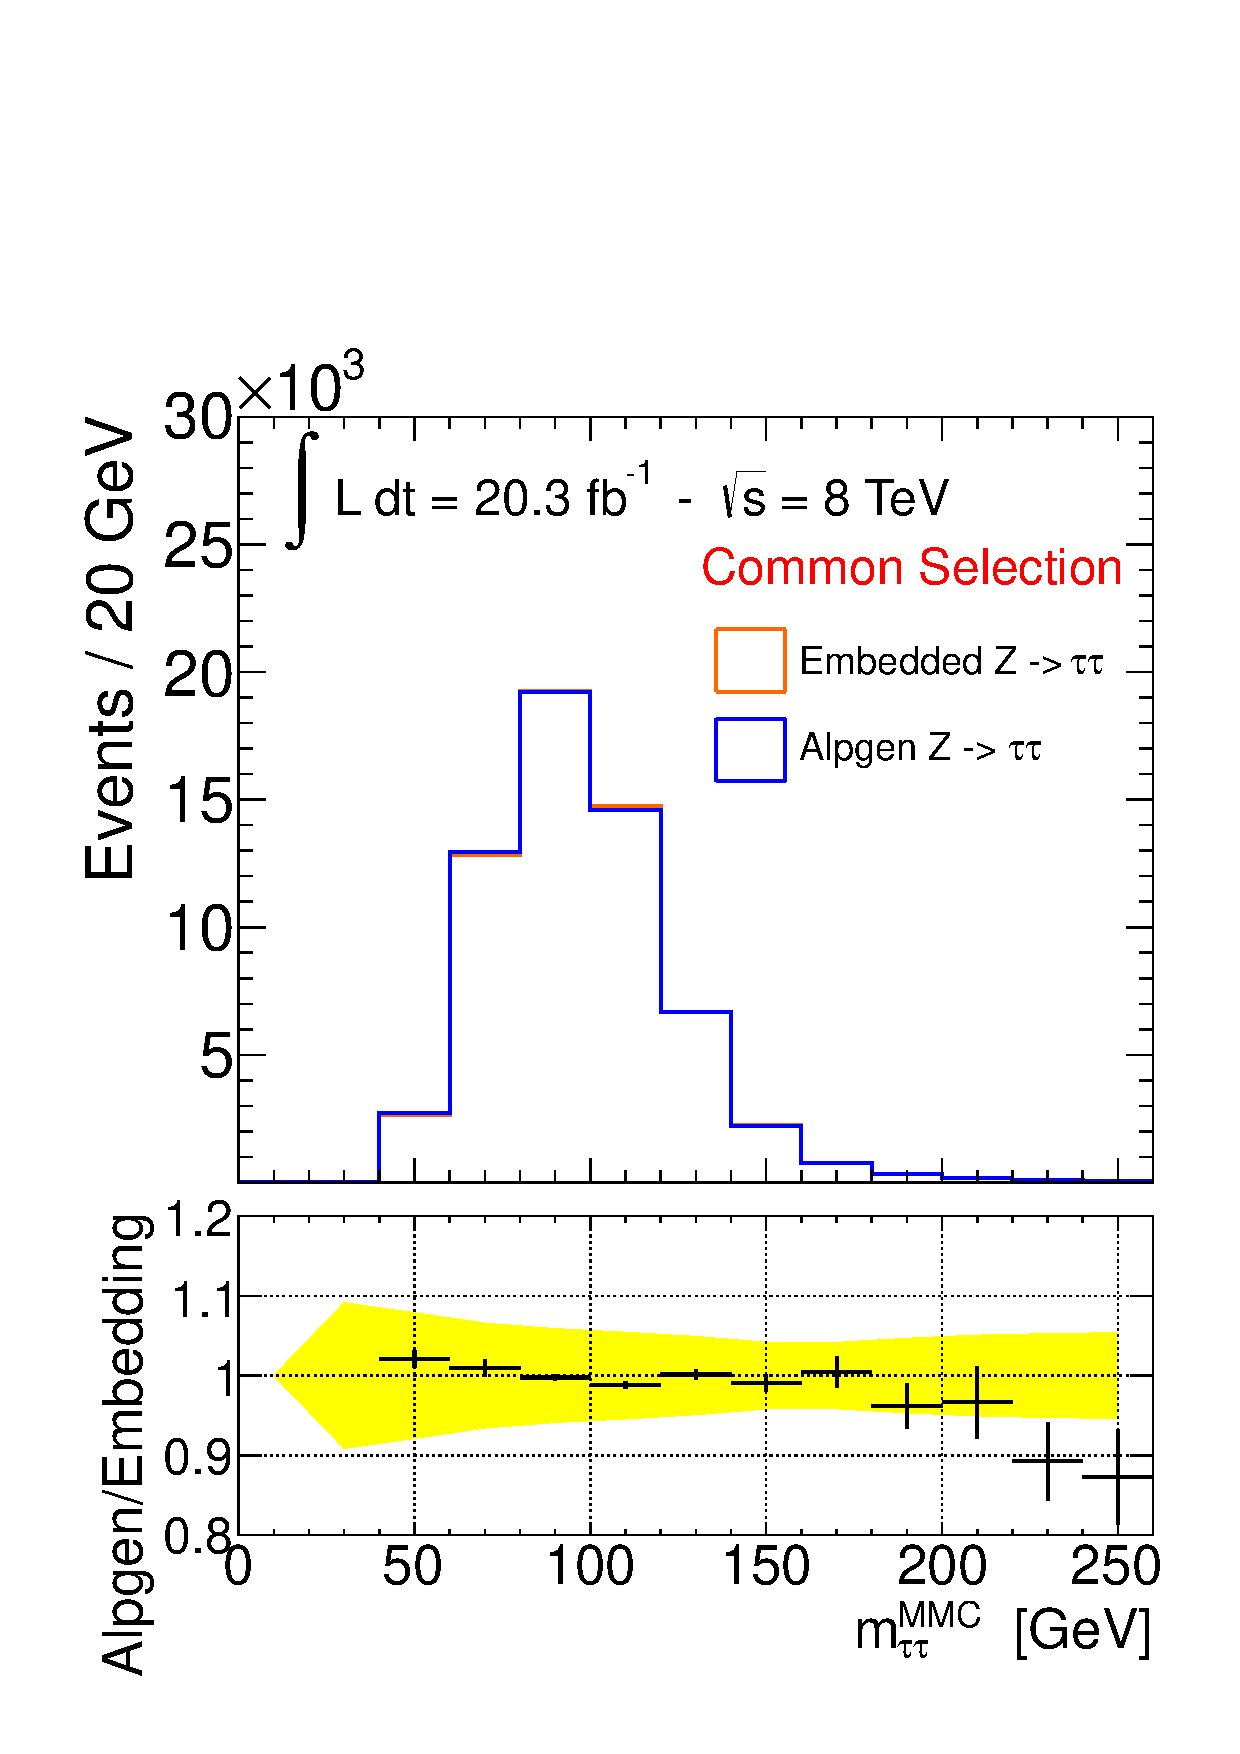
\includegraphics[page=1, width=0.47\textwidth]{figure/emb_plots.pdf}
\end{center}
    \caption{Comparison of the \mmc distributions obtained from the ALPGEN \Ztautau simulation and from the embedding technique after 
	the requirements of th common selection  has been applied. 
	The yellow bad indicates the total systematic uncertainty  relative to the ALPGEN simulation sample.}
   \label{fig:emb_vs_alp1}
\end{figure}

The embedding technique has been validated in several studies detailed in~\cite{Embedding, SMnew}  demonstrating  reliable 
description of the data. Figure~\ref{fig:emb_vs_alp1} shows the excellent agreement between  the \mmc distributions of embedded and 
simulated \Ztautau events. On the other hand, other important variables, such as the \MET
and the number of b-jets in the final state, are  better described by the embedded rather than the 
simulated $\Ztautau$ sample as shown in Figure~\ref{fig:emb_vs_alp}.
This  is expected and is due to the imperfect modelling of these variables in the simulation.


\begin{figure}[tp]
     \begin{center}

           \includegraphics[page=2, width=0.47\textwidth]{figure/emb_plots.pdf}
            \includegraphics[page=3, width=0.47\textwidth]{figure/emb_plots.pdf}

    \end{center}
    \caption{Comparison of the  $\MET$ (left)  and  b-tagged jet multiplicity (right) distributions in
	embedded and in ALPGEN \Ztautau events after the  common selection.
	Data are superimposed after subtracting  the contributions of non-\Ztautau processes.The yellow band indicates
	 the total systematic uncertainty  of the ALPGEN simulation.}
   \label{fig:emb_vs_alp}
\end{figure}

\begin{table} [p]
\begin{footnotesize}
\centering
\begin{tabular}{c c c c c}
\hline
\hline
 & Embedded event yield & Transfer 	& Estimated events	  & Contamination \\
 & in \ttbar control sample & factor&  in signal sample&	 \\ [0.5ex]
\hline
b-taged & $84 \pm 9$  & $(2.6 \pm 0.1) \times 10^{-2}$ &  $2.2 \pm 0.2$&  0.5 \% \\
b-vetoed & $84 \pm 9$ & $(1.74 \pm 0.02) \times 10^{-1}$ & $15 \pm 2$ & 0.03 \% \\[1ex]
\hline
\end{tabular}
\end{footnotesize}
\caption{Evaluation of the $t\bar{t}$ contamination  in the embedded $\Ztt$ sample requiring a two b-tagged jets. 
The transfer factor from the validation sample to the signal sample  is  obtained from simulation. }
\label{table:emb_cont_tt}
\end{table}

\begin{table} [tp]
\begin{footnotesize}
\centering
\begin{tabular}{c c c c c}
\hline
\hline
 & Embedded event yield	& Transfer	& Estimated events	& Contamination \\
 &  in QCD control sample C		& factor	& in signal sample	&	\\		 [0.5ex]
\hline
B-tag  & $12 \pm 3$ & $ (7 \pm 1) \times 10^{-3}$ &  $(8.4 \pm 0.3) \times 10^{-2}$ &  0.03 \% \\
B-veto & $390 \pm 20$ & $(2.5 \pm 0.1) \times 10^{-2}$ & $10.0 \pm 0.5$ & 0.02 \% \\[1ex]
\hline
\end{tabular}
\end{footnotesize}
\caption{Evaluation of the QCD multi-jet contamination  in the embedded $\Ztt$ sample  requiring OS non-isolated leptons
	(sample C). The transfer factor $R_{QCD}^{\mu\mu}$ extrapolates the event yield measured in control sample C to the signal 
	sample (see text).}
\label{table:emb_cont_qcd}
\end{table}


%plot comparing embedding and ALPGEN Et miss and b-tagging, data -MC not Ztautau and compare data alp and ebb.

The embedding method uses selected \Zmumu data events. The \Zmumu selection criteria 
assure a pure \Zmumu sample, however, further event selection criteria used in this analysis, 
for example the b-tagging requirements, can enhance the contamination of this sample. 
Dedicated studies have been made to estimate the $t\bar{t}$ and QCD multi-jet contamination in the embedded sample.
The \ttbar~ contamination is estimated by evaluating the yield of embedded \Ztt events with the additional requirement of 
two b-tagged jets as described in Section~\ref{sec:top_est}. These events are assumed to originate solely from  $t\bar{t}$ production
and the corresponding yield in the signal sample is determined by extrapolation using the simulation.
Table~\ref{table:emb_cont_tt} summarises the estimated top quark contamination in the embedded $\Ztt$ sample
 separately for the two event categories.
The multi-jet contamination is estimated in a similar way  starting 
from the yield of embedded events in  sample C of the ABCD method. 
%one should not use SS samples because embedding already requires leptons to be OS, then would be biased
It is assumed that all events in this validation sample are QCD multi-jet events. The QCD multi-jet contamination 
of the embedded events in the  signal region A is estimated as
\begin{equation} \label{eqn:qcdEmb}
N_{A}^{QCD-emb}  = N_{C}^{QCD-emb} \times \frac{N_{B}^{\mu\mu}}{N_{D}^{\mu\mu}} =  N_{B} \times R_{QCD}^{\mu\mu} \,.
\end{equation}
The transfer factor $R_{QCD}^{\mu\mu}$ is evaluated using a di-muon final state with the same kinematical selection criteria
 as for the \Zmumu candidates used for  the embedding procedure.
Table~\ref{table:emb_cont_qcd} shows the estimated contamination of embedded sample with QCD multi-jet events
which is considered negligible.




